% !TEX encoding = UTF-8 Unicode
% !TEX root = ../report.tex
% 
\section{Gráficas}
\label{graficas}

En este apéndice se incluyen todas las gráficas obtenidas a partir de las muestras obtenidas para el \nameref{analisis}
(en la sección \ref{analisis}).

En el apéndice \ref{tablas} se pueden encontrar todas las tablas que resumen las gráficas que aquí se presentan.

\subsection{Memoria fijada a 1024 bytes}

\forloop{dataset}{1}{\value{dataset} < 10}{

\subsubsection{\emph{Dataset} D\arabic{dataset}.dat}
\begin{figure}[h!]
    \centering
        \includegraphics[width=0.64\textwidth]{../figs/D\arabic{dataset}/plot_estimation_1024.pdf}
        \caption{Estimaciones por cada ejecución en el dataset D\arabic{dataset}.dat}
    \label{figura:D\arabic{dataset}_estimation}
\end{figure}

\begin{figure}[h!]
    \centering
        \includegraphics[width=0.64\textwidth]{../figs/D\arabic{dataset}/plot_errors_1024.pdf}
        \caption{Errores relativos por cada ejecución en el dataset D\arabic{dataset}.dat}
    \label{figura:D\arabic{dataset}_errors}
\end{figure}

\begin{figure}[h!]
    \centering
        \includegraphics[width=0.64\textwidth]{../figs/D\arabic{dataset}/plot_count_1024.pdf}
        \caption{Clasificación de ejecuciones según error relativo en el dataset D\arabic{dataset}.dat}
    \label{figura:D\arabic{dataset}_count}
\end{figure}

\begin{figure}[h!]
    \centering
        \includegraphics[width=0.64\textwidth]{../figs/D\arabic{dataset}/plot_time_1024.pdf}
        \caption{Tiempos de ejecución en el dataset D\arabic{dataset}.dat}
    \label{figura:D\arabic{dataset}_time}
\end{figure}

\clearpage

}

\subsection{Influencia de la memoria disponible}

\subsubsection{32 bytes}
\begin{figure}[h!]
    \centering
        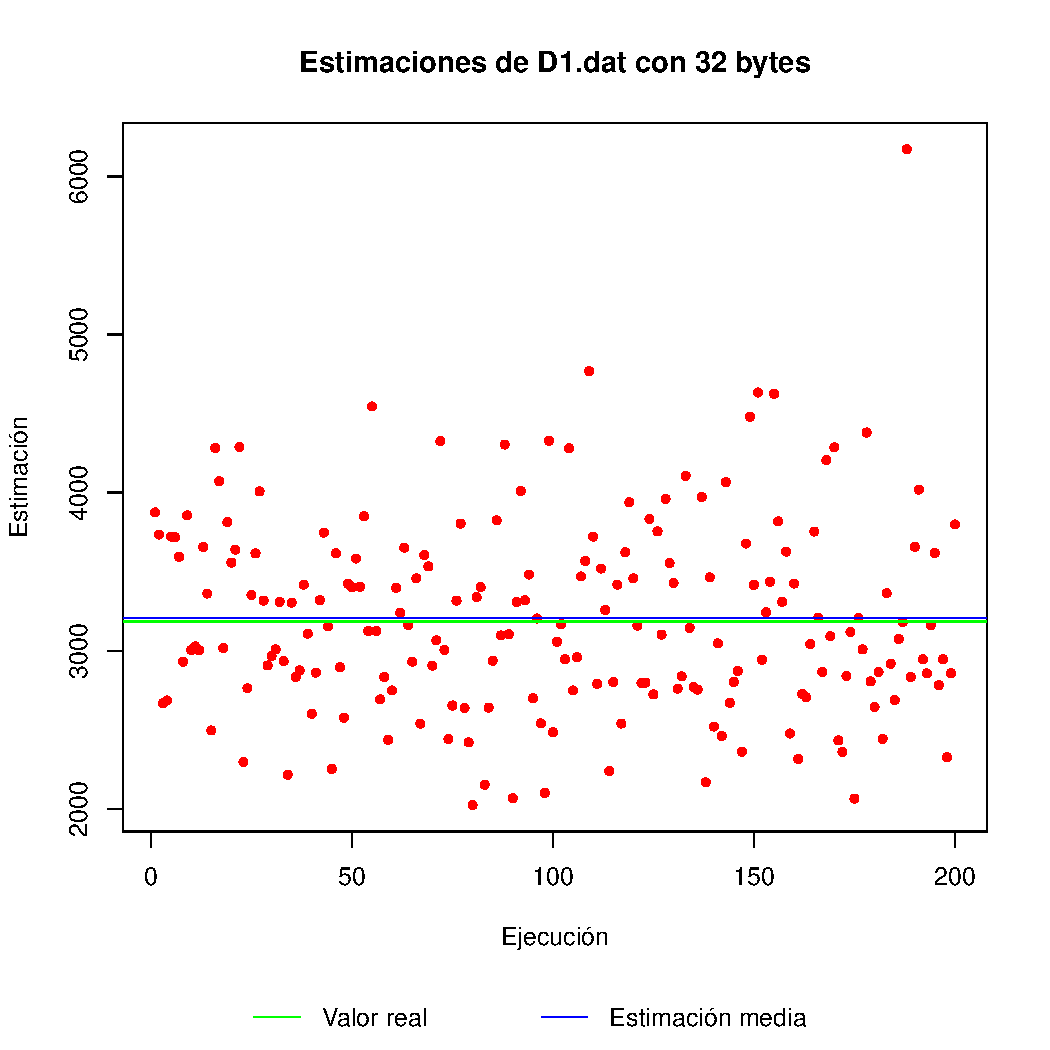
\includegraphics[width=0.64\textwidth]{../figs/D1/plot_estimation_32.pdf}
        \caption{Estimaciones en D1.dat con 32 bytes}
    \label{figura:D1_estimation_32}
\end{figure}

\begin{figure}[h!]
    \centering
        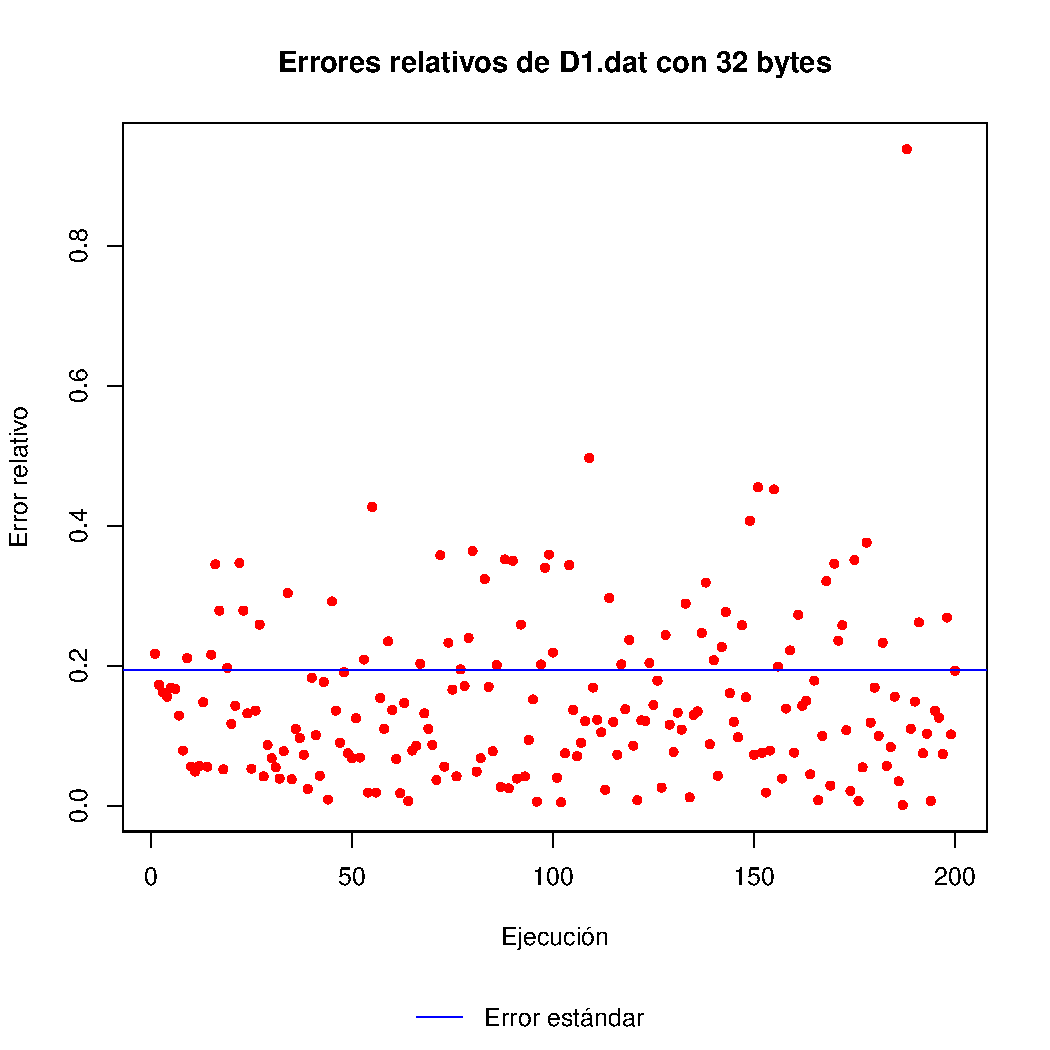
\includegraphics[width=0.64\textwidth]{../figs/D1/plot_errors_32.pdf}
        \caption{Errores relativos en D1.dat con 32 bytes}
    \label{figura:D1_errors_32}
\end{figure}

\begin{figure}[h!]
    \centering
        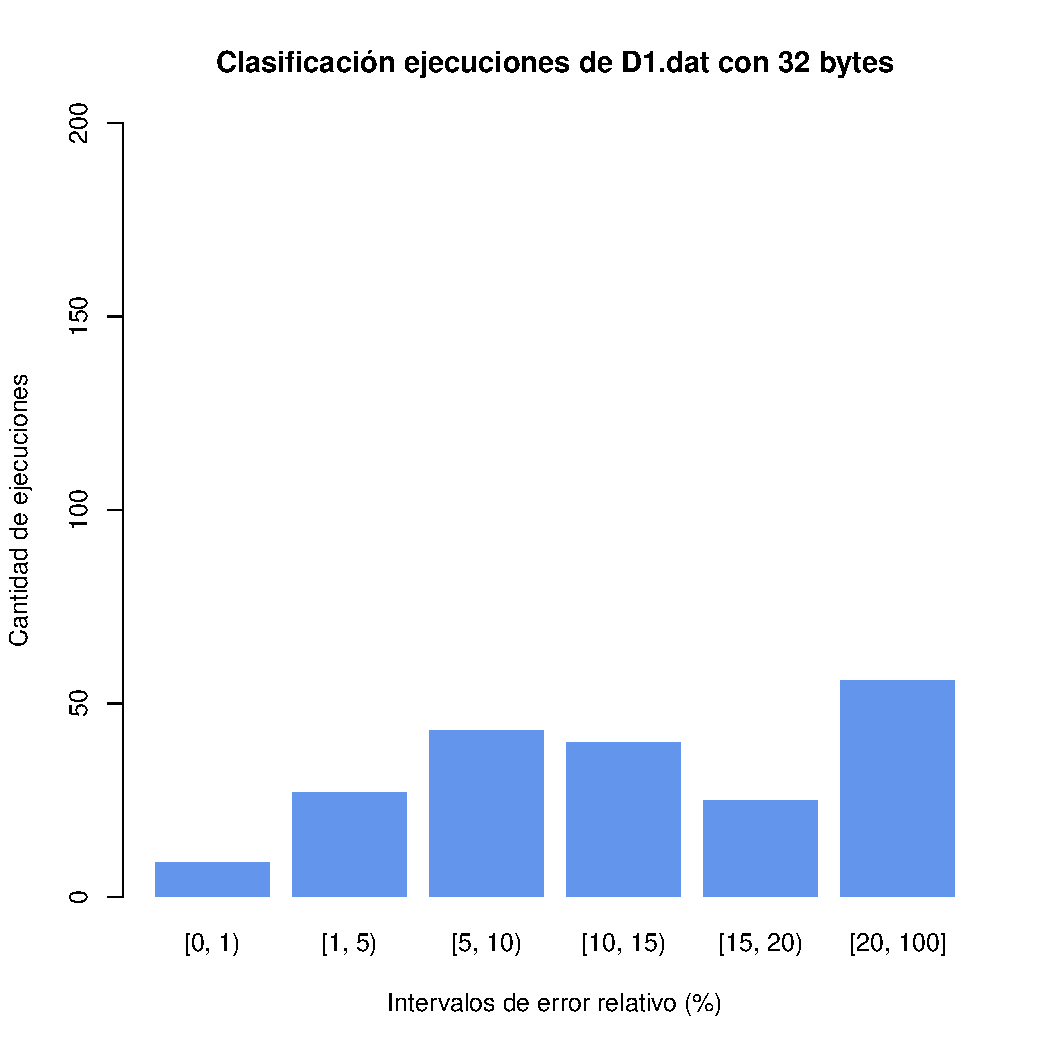
\includegraphics[width=0.64\textwidth]{../figs/D1/plot_count_32.pdf}
        \caption{Clasificación de ejecuciones en D1.dat con 32 bytes}
    \label{figura:D1_count_32}
\end{figure}

\begin{figure}[h!]
    \centering
        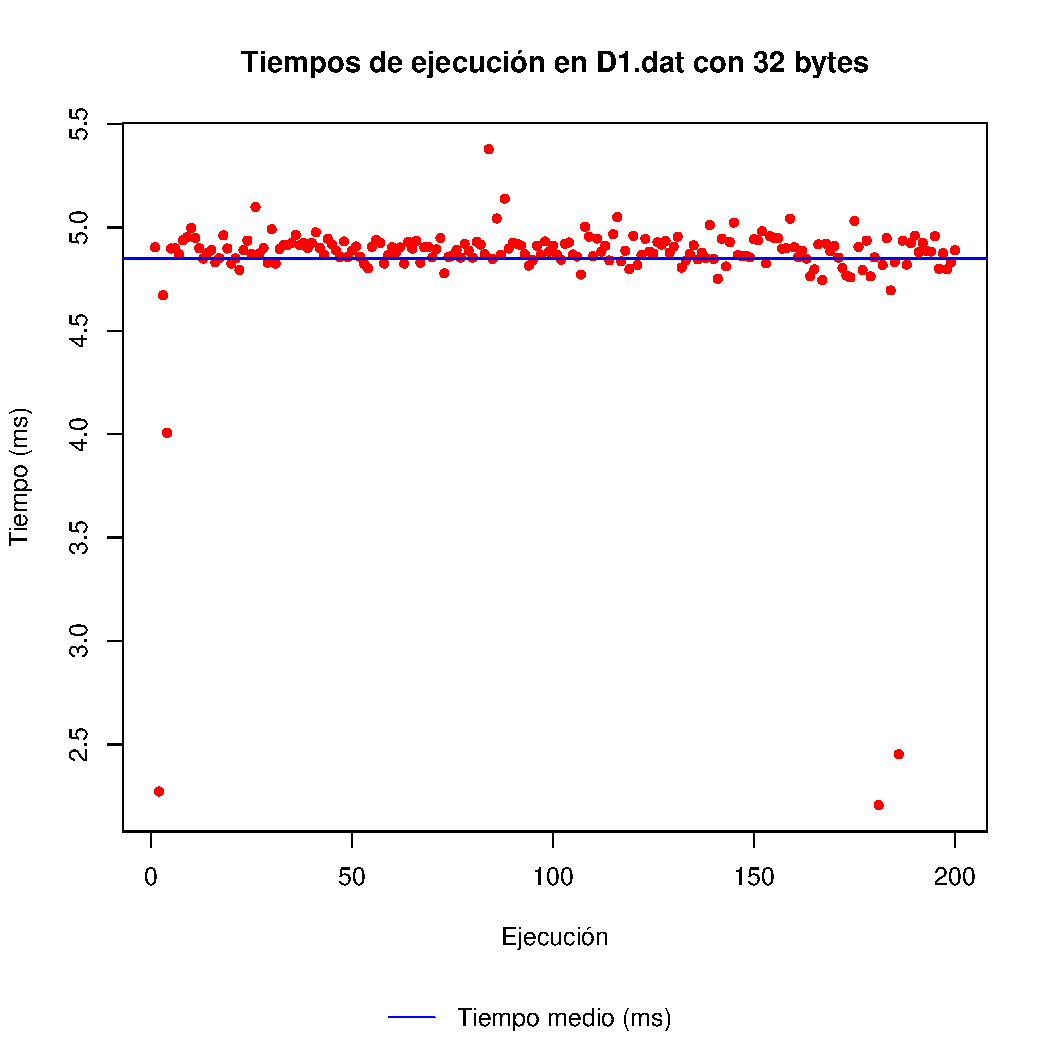
\includegraphics[width=0.64\textwidth]{../figs/D1/plot_time_32.pdf}
        \caption{Tiempos de ejecución en D1.dat con 32 bytes}
    \label{figura:D1_time_32}
\end{figure}

\clearpage
\subsubsection{64 bytes}
\begin{figure}[h!]
    \centering
        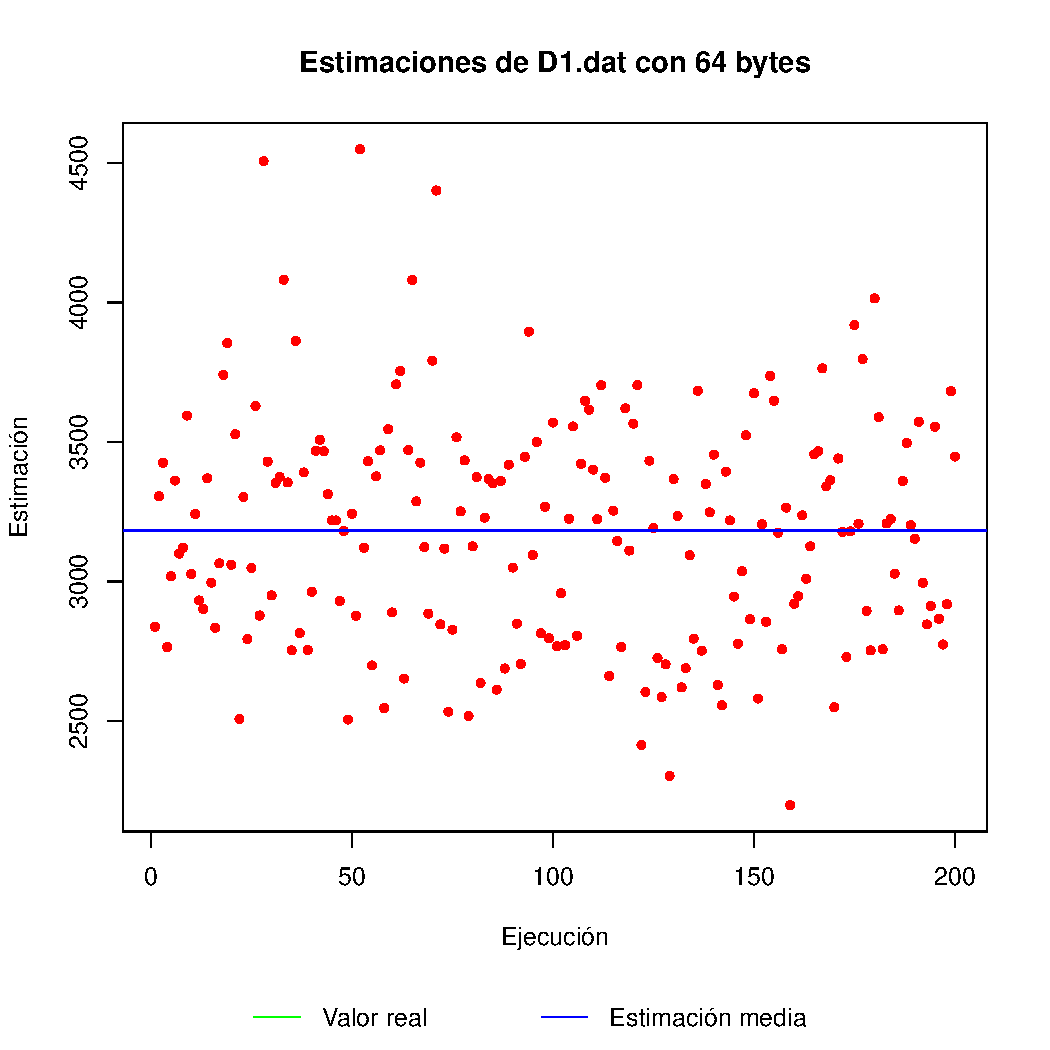
\includegraphics[width=0.64\textwidth]{../figs/D1/plot_estimation_64.pdf}
        \caption{Estimaciones en D1.dat con 64 bytes}
    \label{figura:D1_estimation_64}
\end{figure}

\begin{figure}[h!]
    \centering
        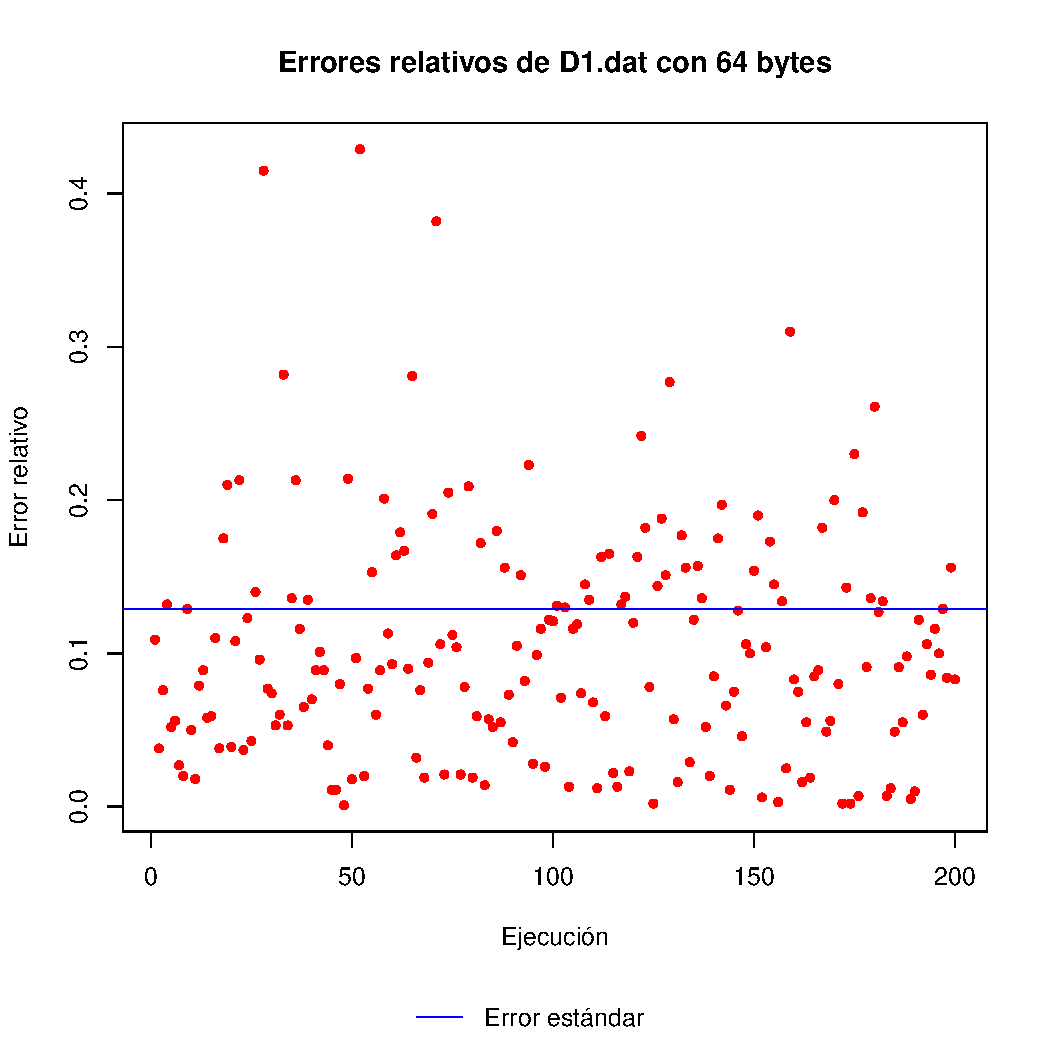
\includegraphics[width=0.64\textwidth]{../figs/D1/plot_errors_64.pdf}
        \caption{Errores relativos en D1.dat con 64 bytes}
    \label{figura:D1_errors_64}
\end{figure}

\begin{figure}[h!]
    \centering
        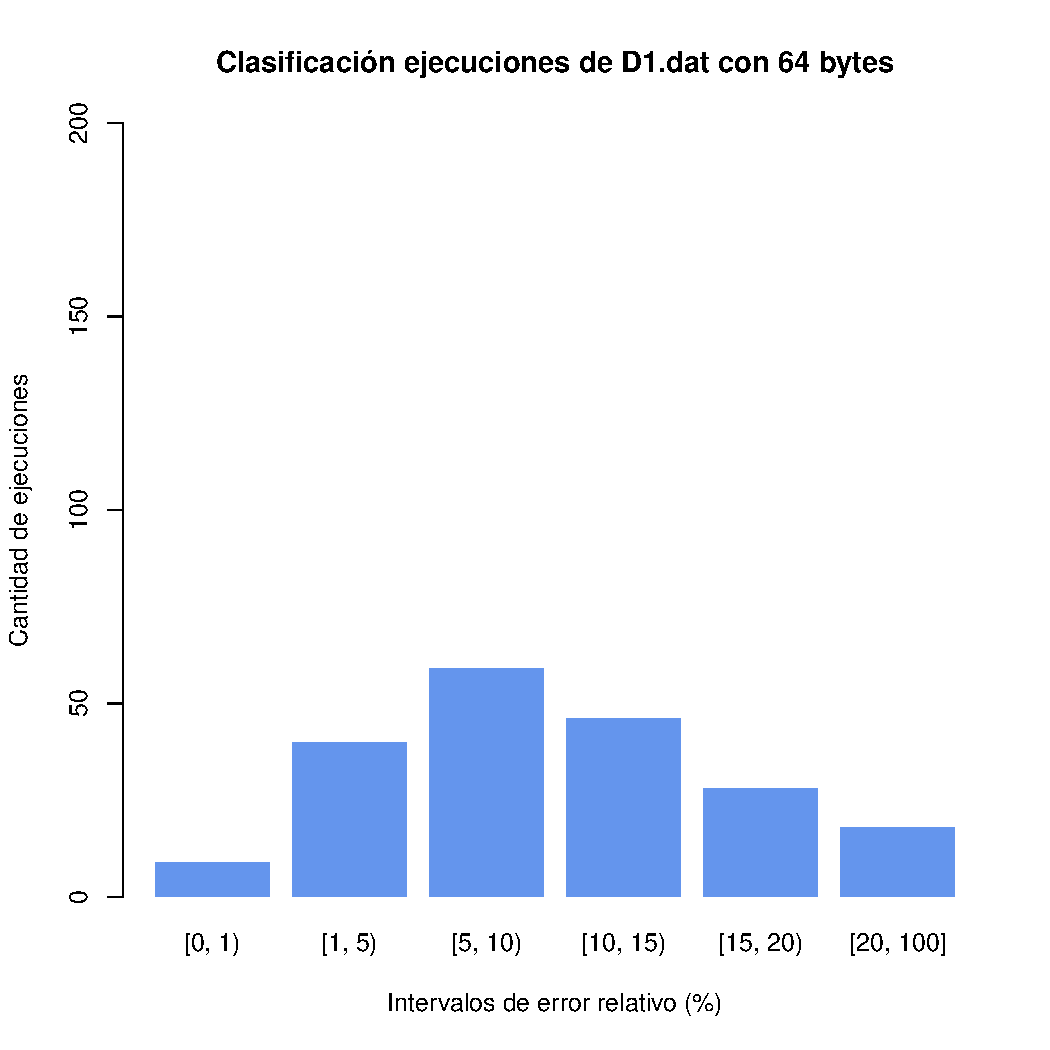
\includegraphics[width=0.64\textwidth]{../figs/D1/plot_count_64.pdf}
        \caption{Clasificación de ejecuciones en D1.dat con 64 bytes}
    \label{figura:D1_count_64}
\end{figure}

\begin{figure}[h!]
    \centering
        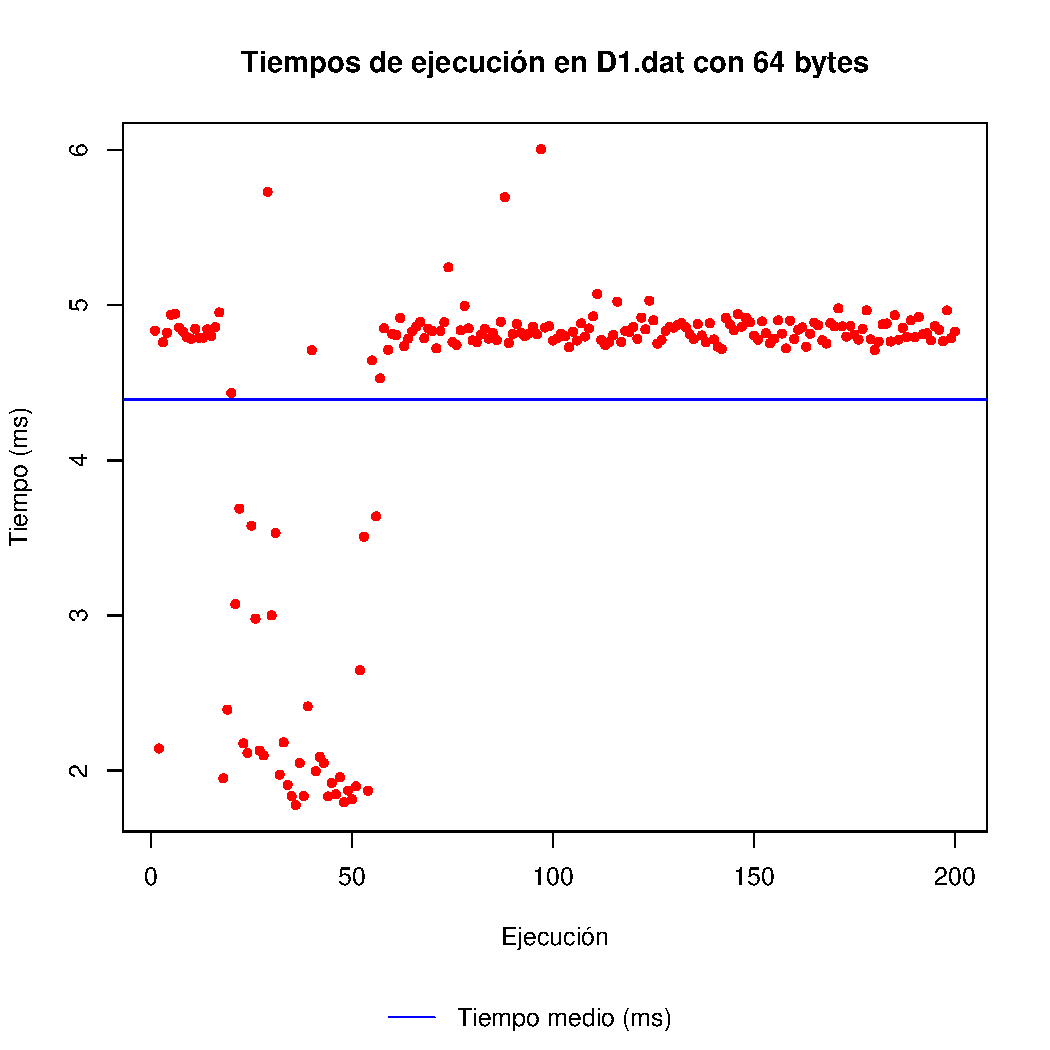
\includegraphics[width=0.64\textwidth]{../figs/D1/plot_time_64.pdf}
        \caption{Tiempos de ejecución en D1.dat con 64 bytes}
    \label{figura:D1_time_64}
\end{figure}

\clearpage
\subsubsection{128 bytes}
\begin{figure}[h!]
    \centering
        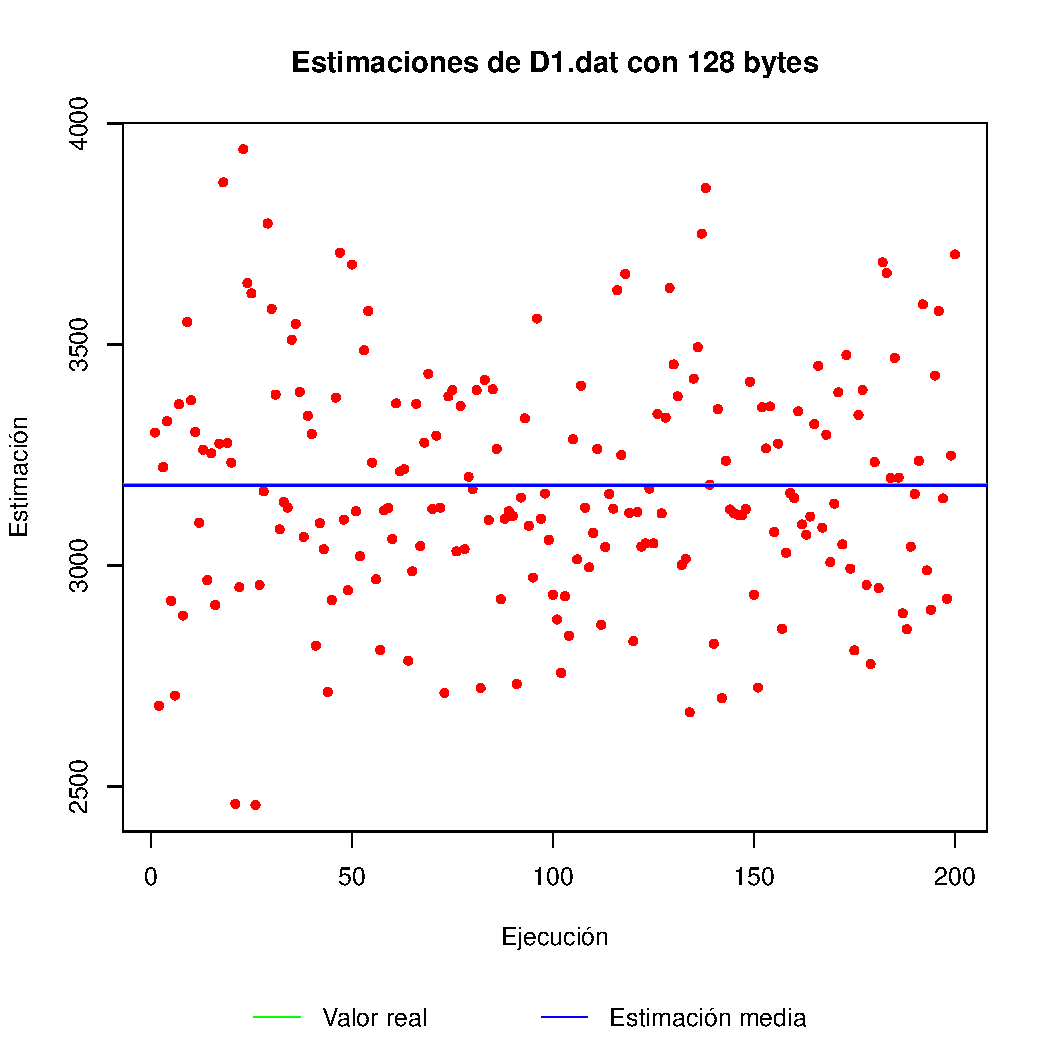
\includegraphics[width=0.64\textwidth]{../figs/D1/plot_estimation_128.pdf}
        \caption{Estimaciones en D1.dat con 128 bytes}
    \label{figura:D1_estimation_128}
\end{figure}

\begin{figure}[h!]
    \centering
        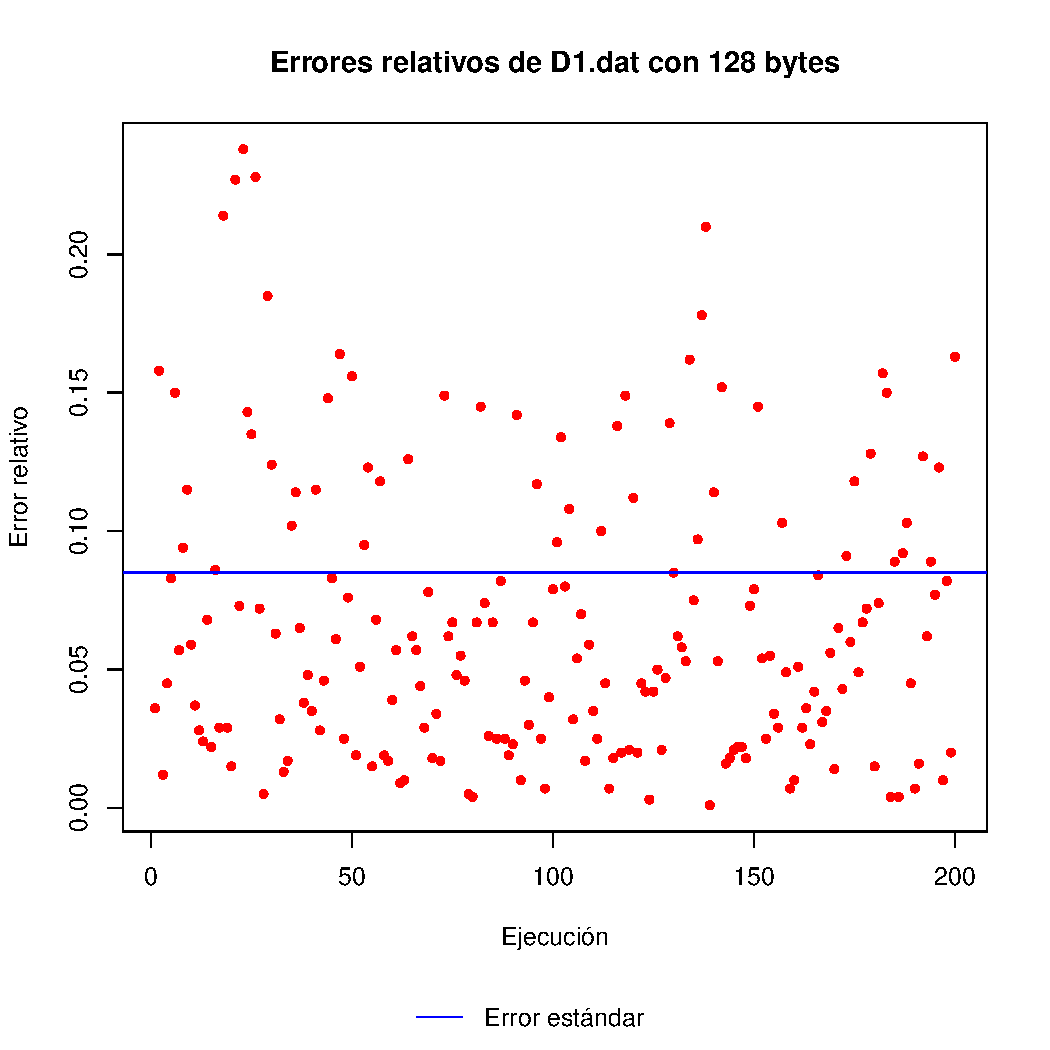
\includegraphics[width=0.64\textwidth]{../figs/D1/plot_errors_128.pdf}
        \caption{Errores relativos en D1.dat con 128 bytes}
    \label{figura:D1_errors_128}
\end{figure}

\begin{figure}[h!]
    \centering
        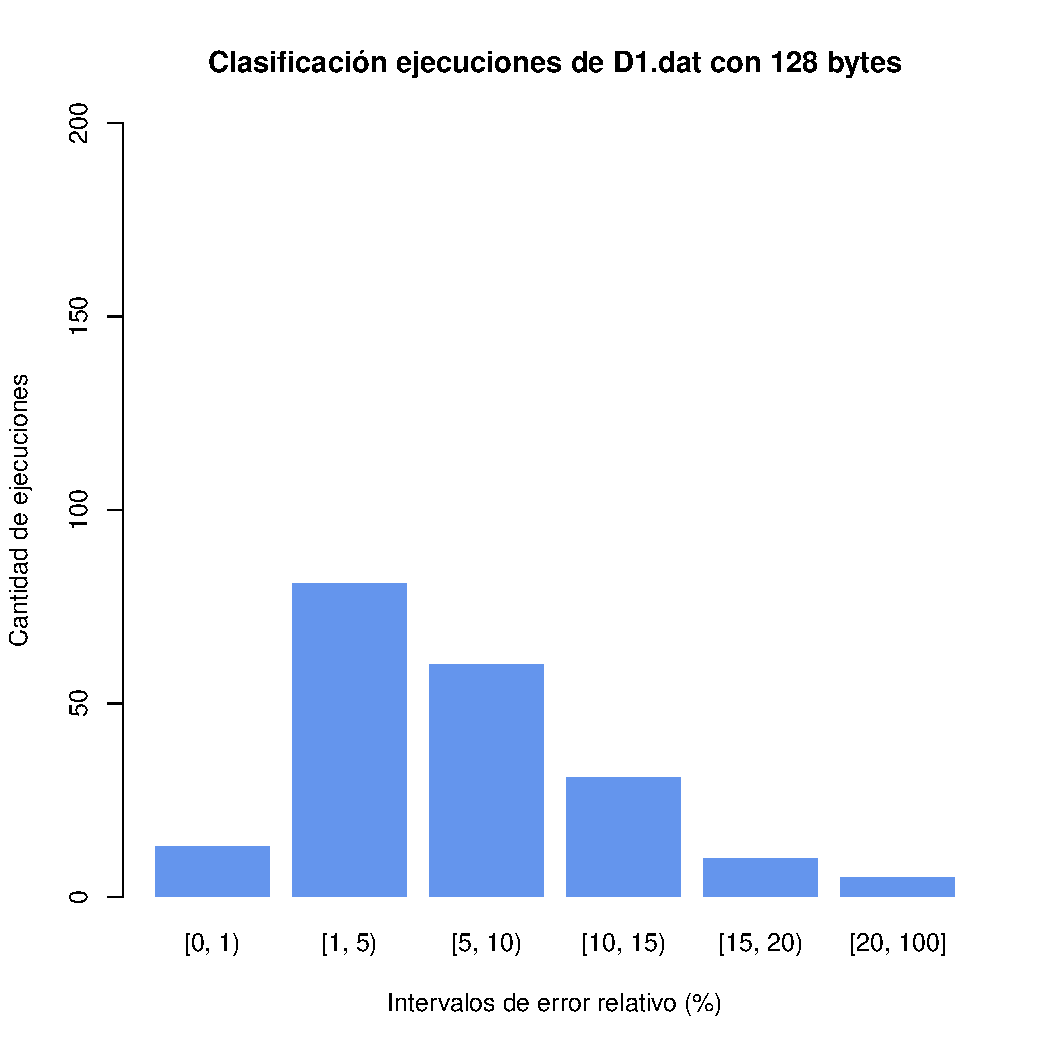
\includegraphics[width=0.64\textwidth]{../figs/D1/plot_count_128.pdf}
        \caption{Clasificación de ejecuciones en D1.dat con 128 bytes}
    \label{figura:D1_count_128}
\end{figure}

\begin{figure}[h!]
    \centering
        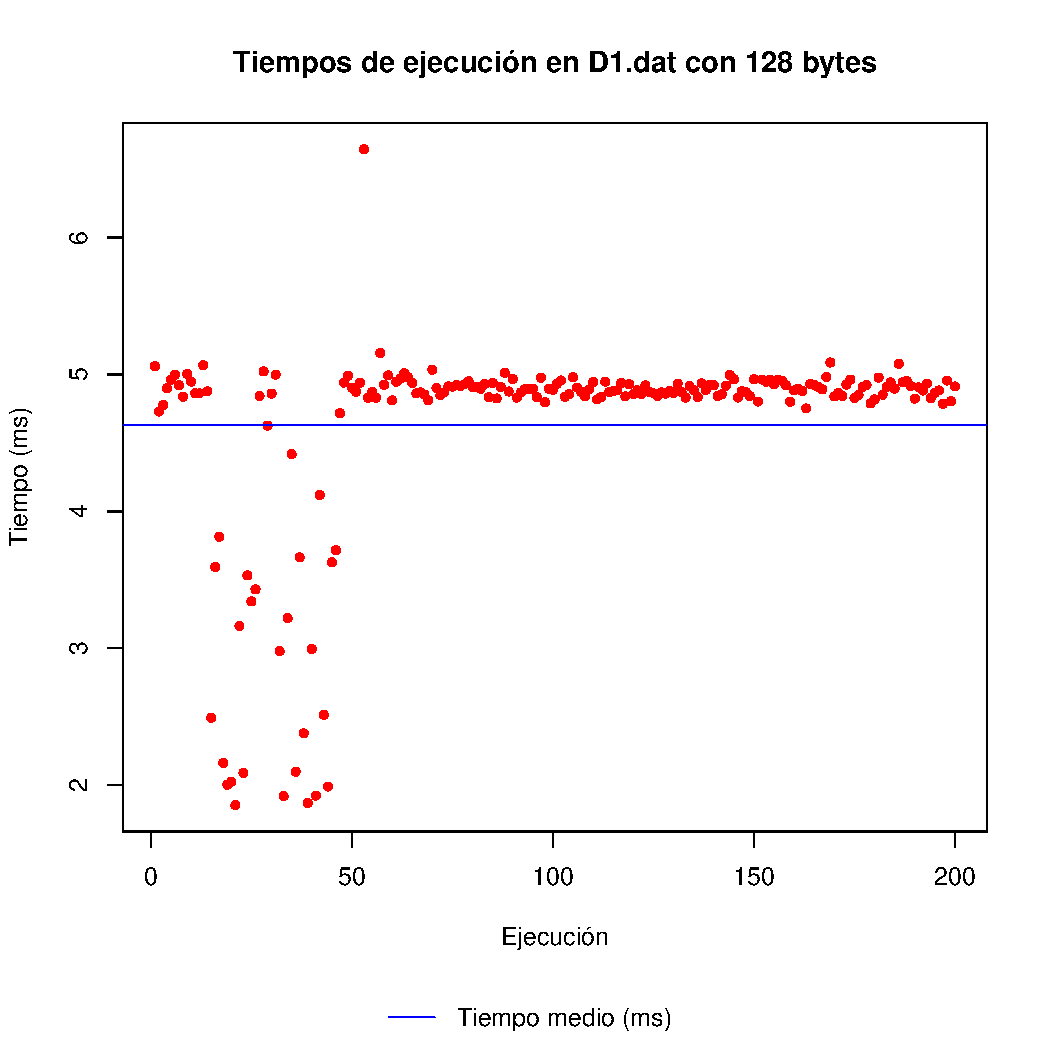
\includegraphics[width=0.64\textwidth]{../figs/D1/plot_time_128.pdf}
        \caption{Tiempos de ejecución en D1.dat con 128 bytes}
    \label{figura:D1_time_128}
\end{figure}

\clearpage
\subsubsection{256 bytes}
\begin{figure}[h!]
    \centering
        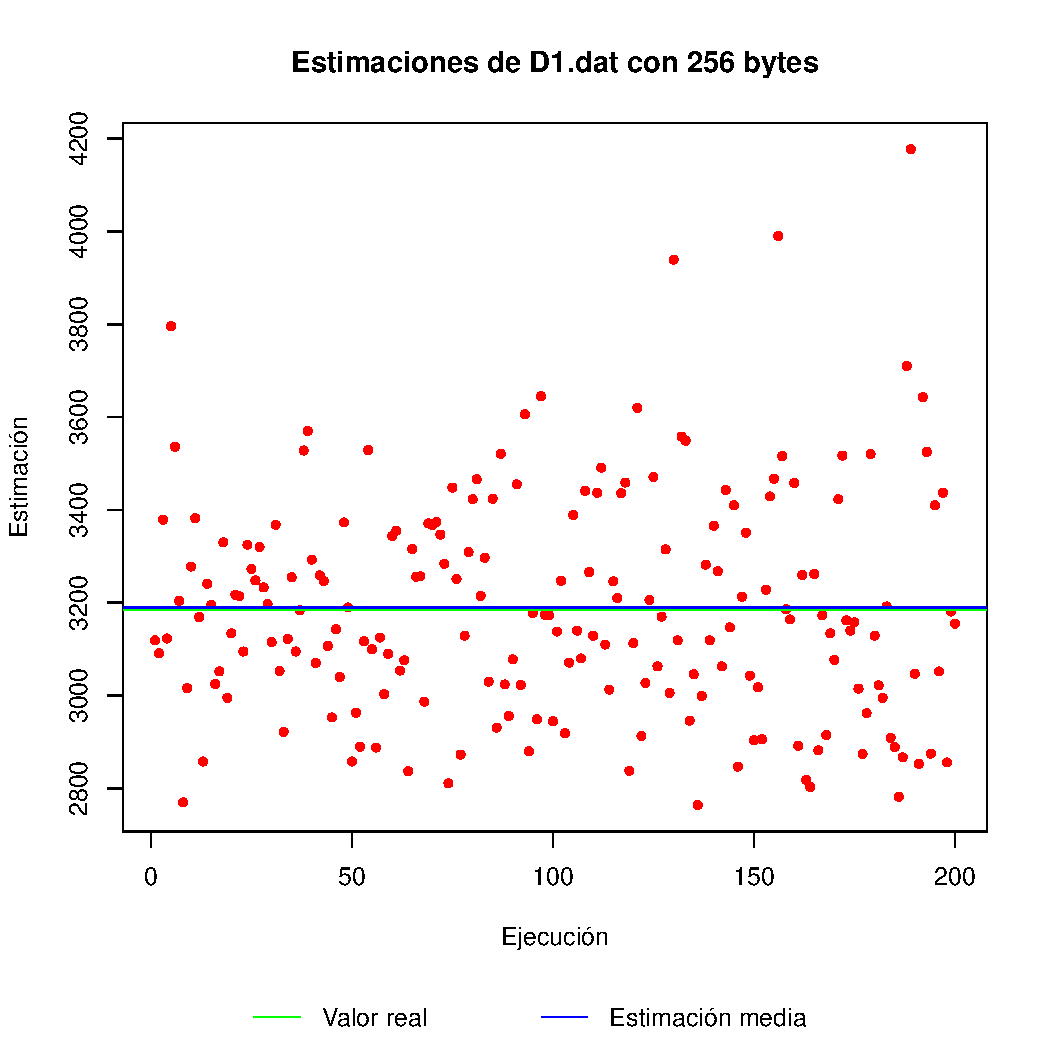
\includegraphics[width=0.64\textwidth]{../figs/D1/plot_estimation_256.pdf}
        \caption{Estimaciones en D1.dat con 256 bytes}
    \label{figura:D1_estimation_256}
\end{figure}

\begin{figure}[h!]
    \centering
        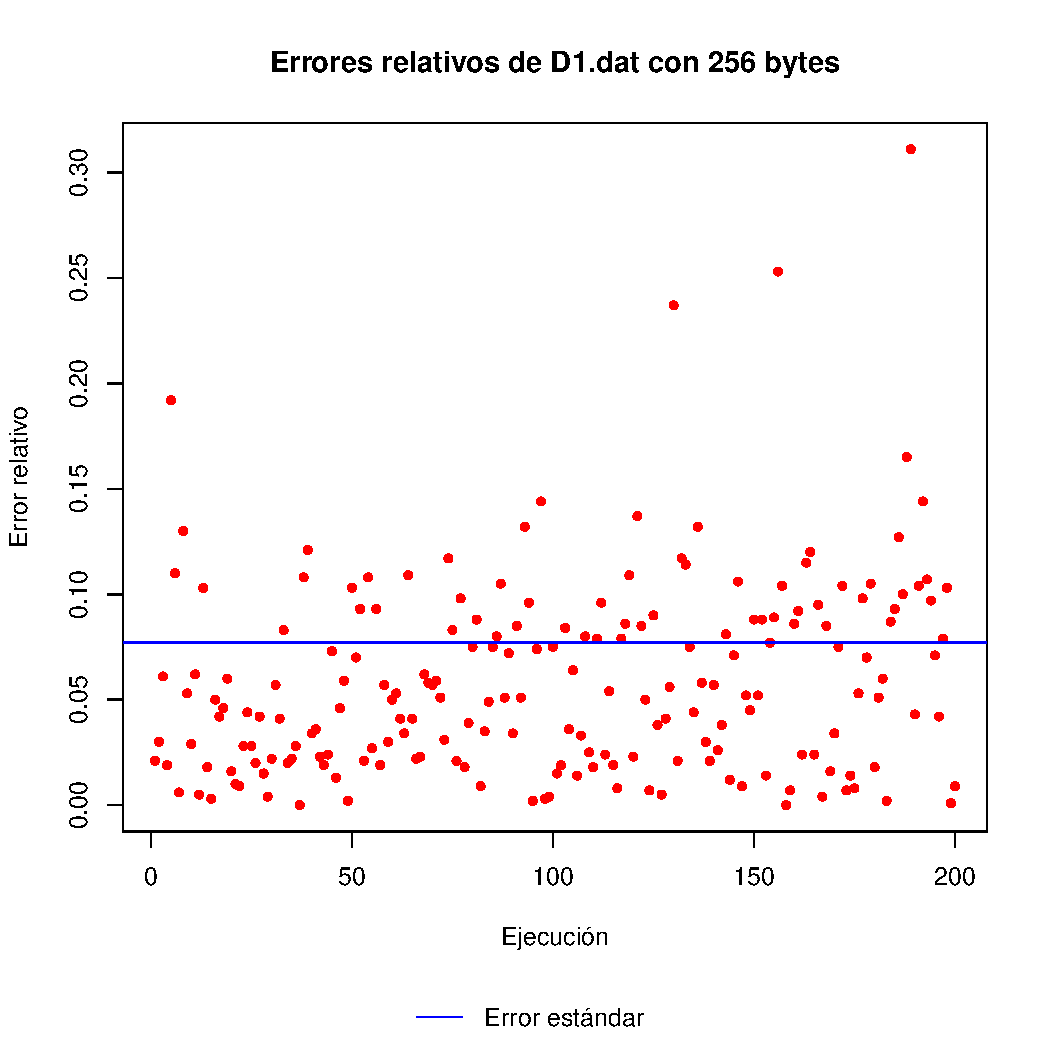
\includegraphics[width=0.64\textwidth]{../figs/D1/plot_errors_256.pdf}
        \caption{Errores relativos en D1.dat con 256 bytes}
    \label{figura:D1_errors_256}
\end{figure}

\begin{figure}[h!]
    \centering
        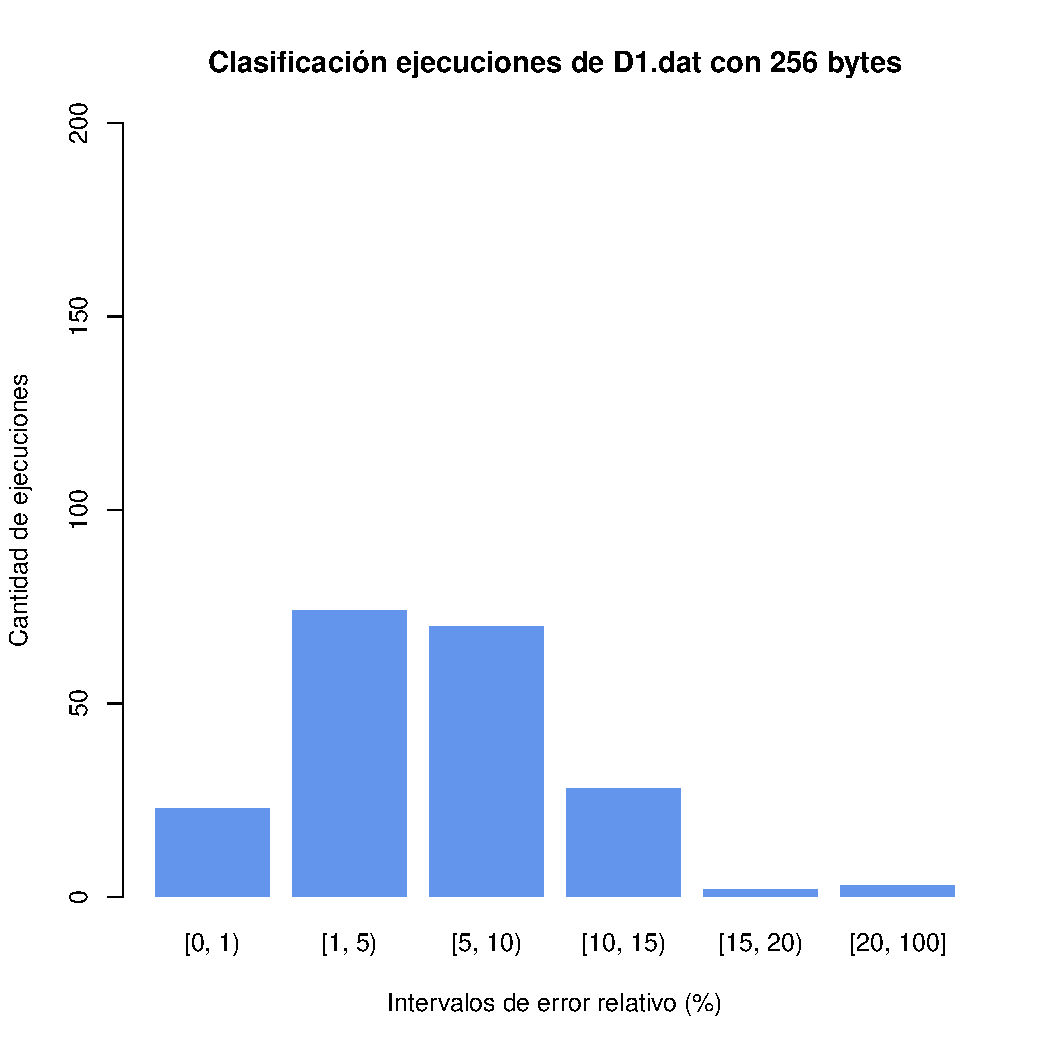
\includegraphics[width=0.64\textwidth]{../figs/D1/plot_count_256.pdf}
        \caption{Clasificación de ejecuciones en D1.dat con 256 bytes}
    \label{figura:D1_count_256}
\end{figure}

\begin{figure}[h!]
    \centering
        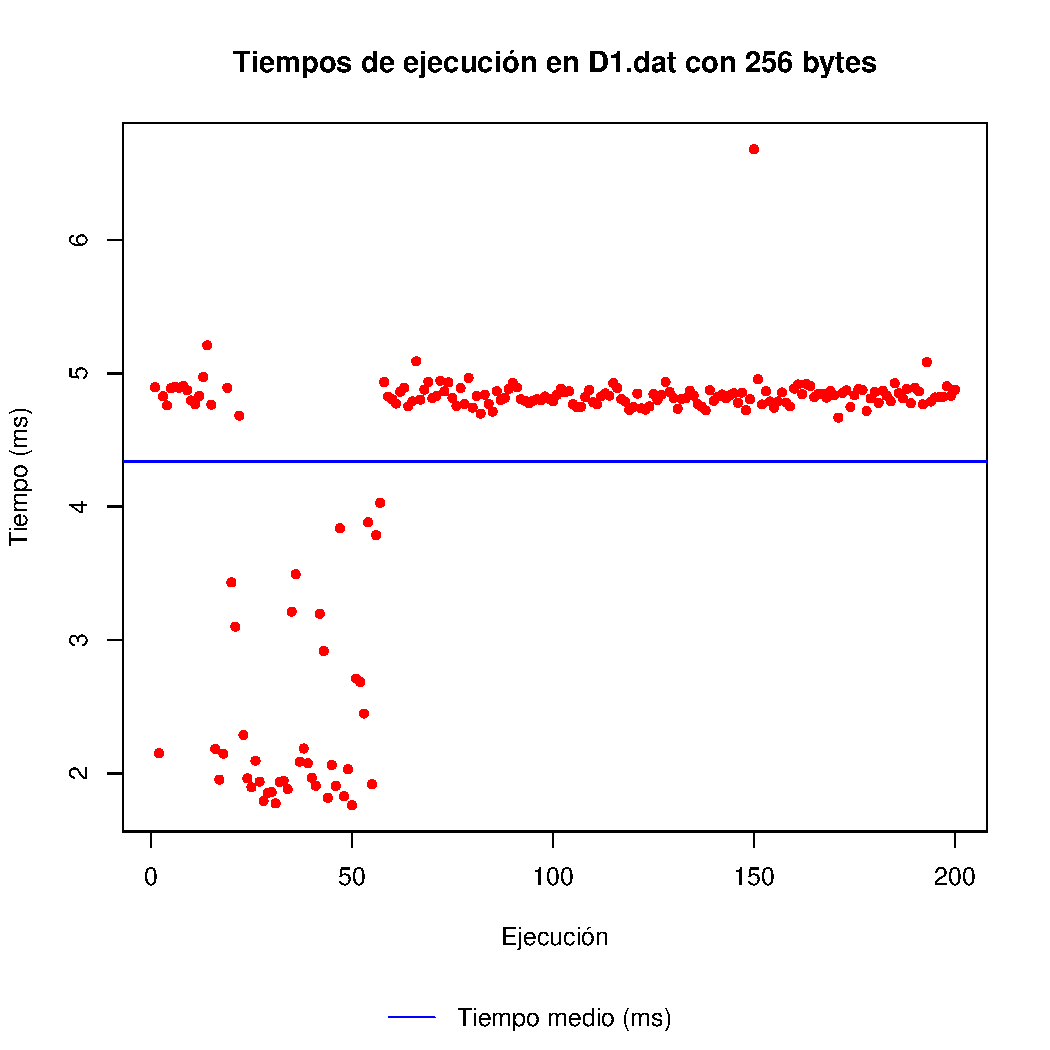
\includegraphics[width=0.64\textwidth]{../figs/D1/plot_time_256.pdf}
        \caption{Tiempos de ejecución en D1.dat con 256 bytes}
    \label{figura:D1_time_256}
\end{figure}

\clearpage
\subsubsection{512 bytes}
\begin{figure}[h!]
    \centering
        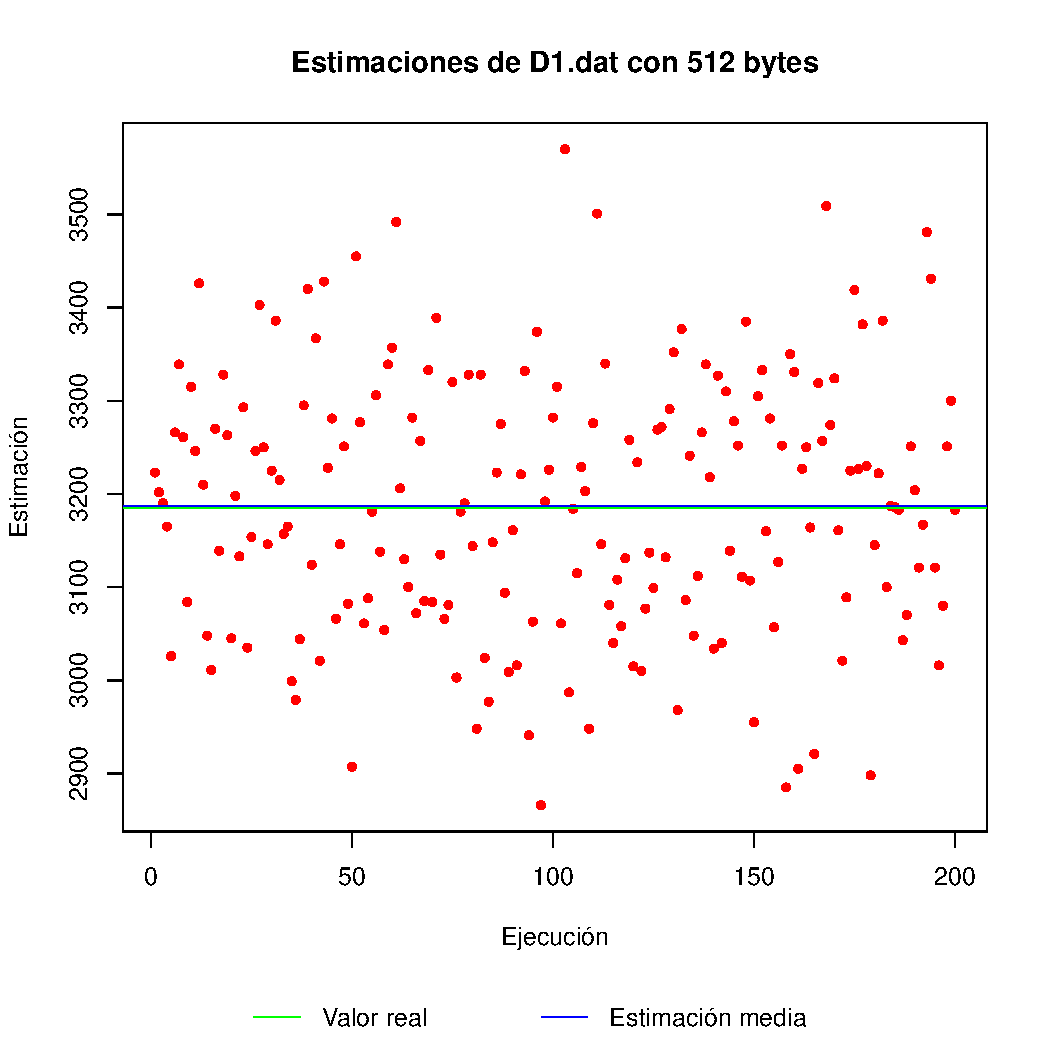
\includegraphics[width=0.64\textwidth]{../figs/D1/plot_estimation_512.pdf}
        \caption{Estimaciones en D1.dat con 512 bytes}
    \label{figura:D1_estimation_512}
\end{figure}

\begin{figure}[h!]
    \centering
        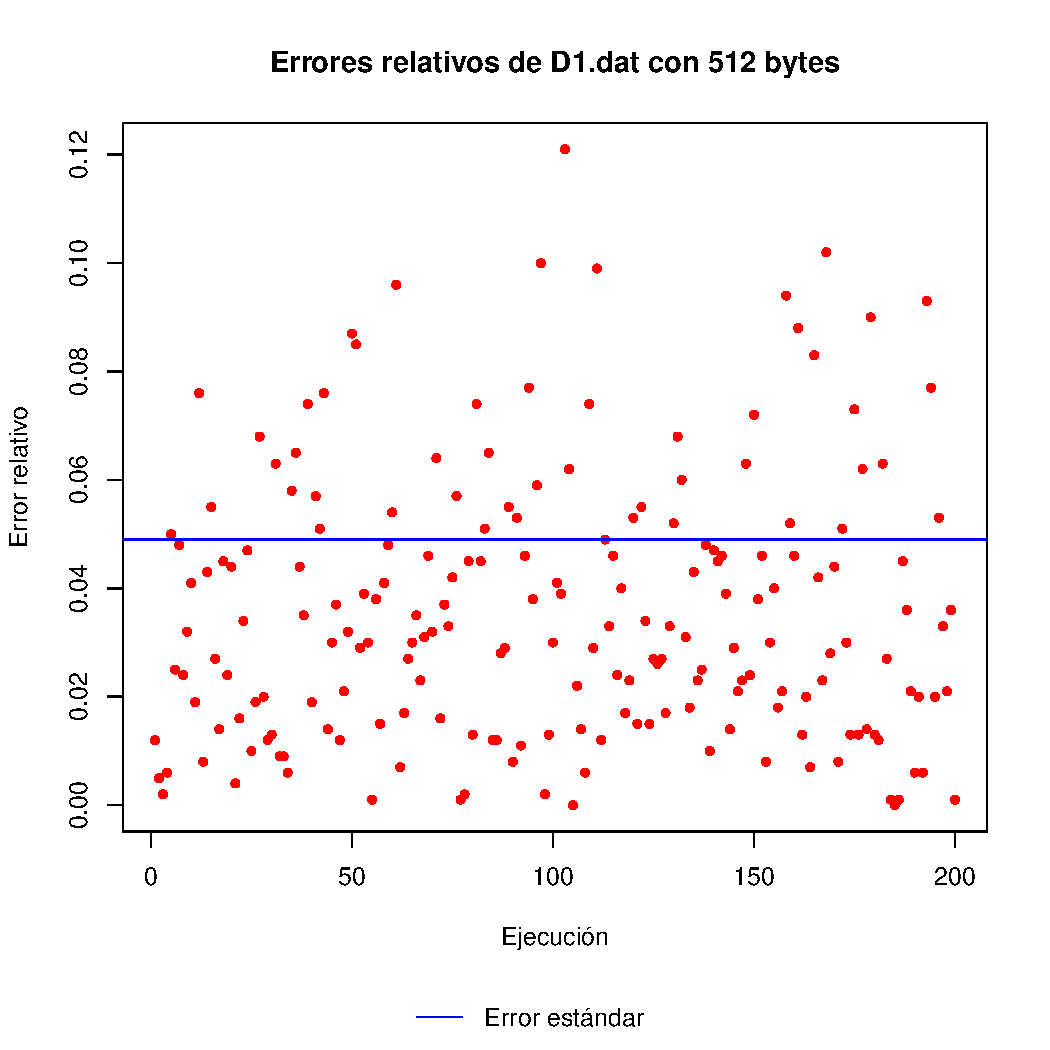
\includegraphics[width=0.64\textwidth]{../figs/D1/plot_errors_512.pdf}
        \caption{Errores relativos en D1.dat con 512 bytes}
    \label{figura:D1_errors_512}
\end{figure}

\begin{figure}[h!]
    \centering
        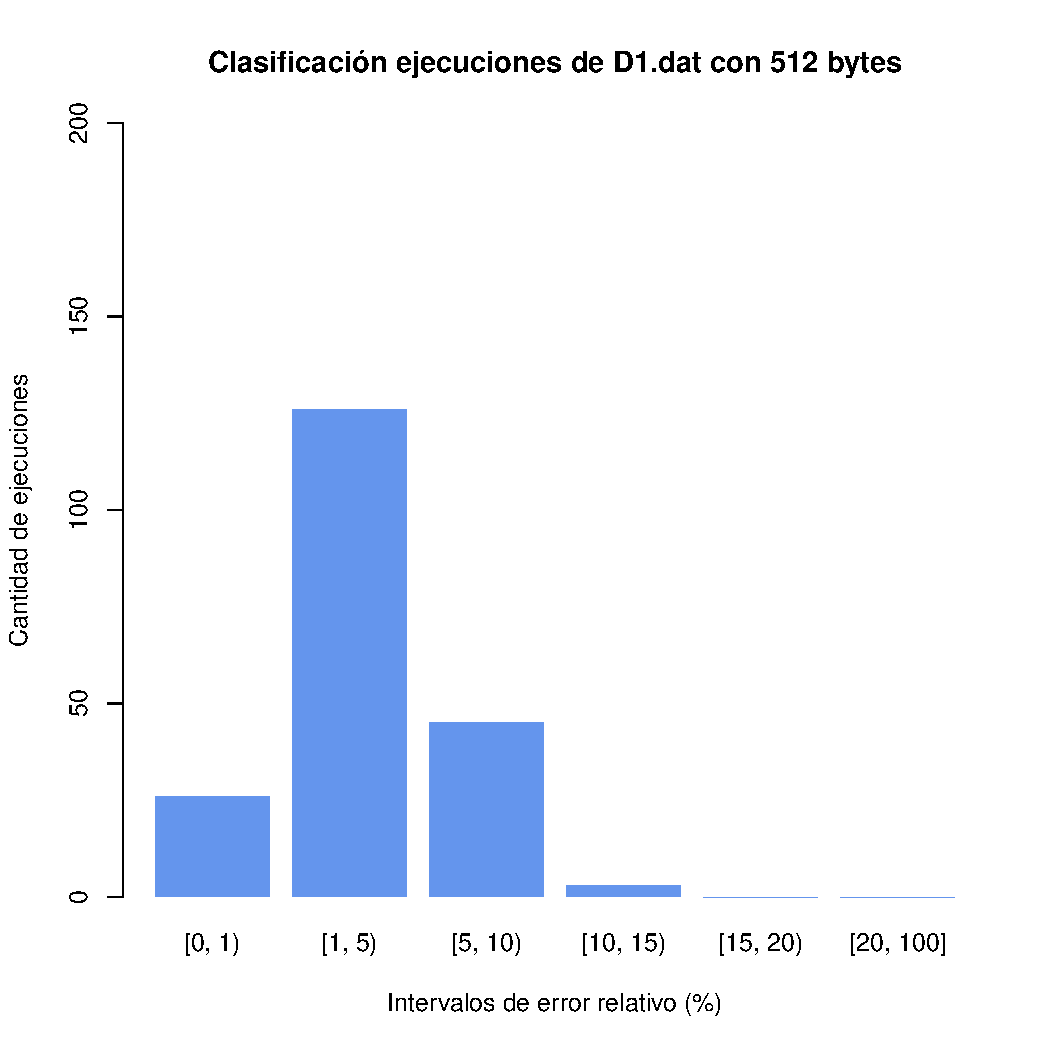
\includegraphics[width=0.64\textwidth]{../figs/D1/plot_count_512.pdf}
        \caption{Clasificación de ejecuciones en D1.dat con 512 bytes}
    \label{figura:D1_count_512}
\end{figure}

\begin{figure}[h!]
    \centering
        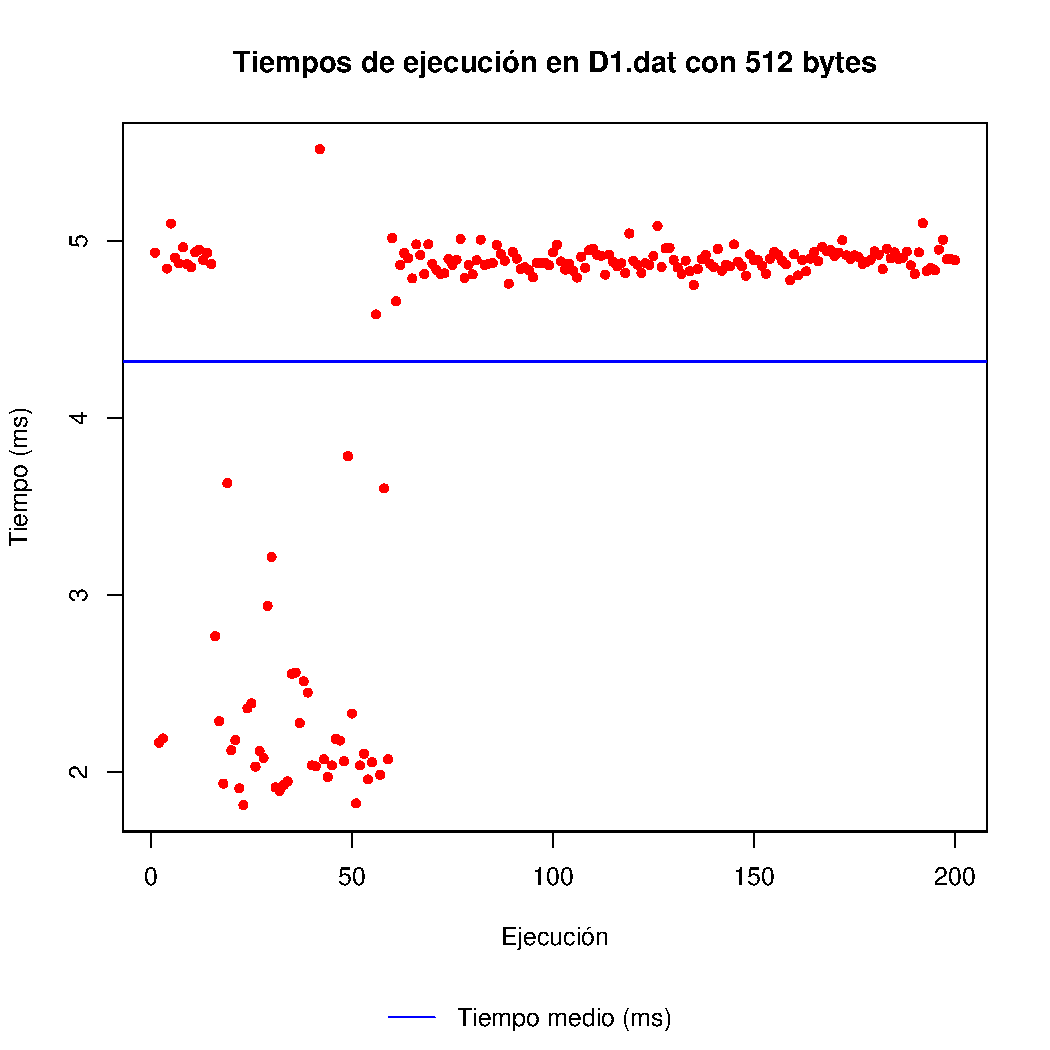
\includegraphics[width=0.64\textwidth]{../figs/D1/plot_time_512.pdf}
        \caption{Tiempos de ejecución en D1.dat con 512 bytes}
    \label{figura:D1_time_512}
\end{figure}

\clearpage
\subsubsection{1024 bytes}
\begin{figure}[h!]
    \centering
        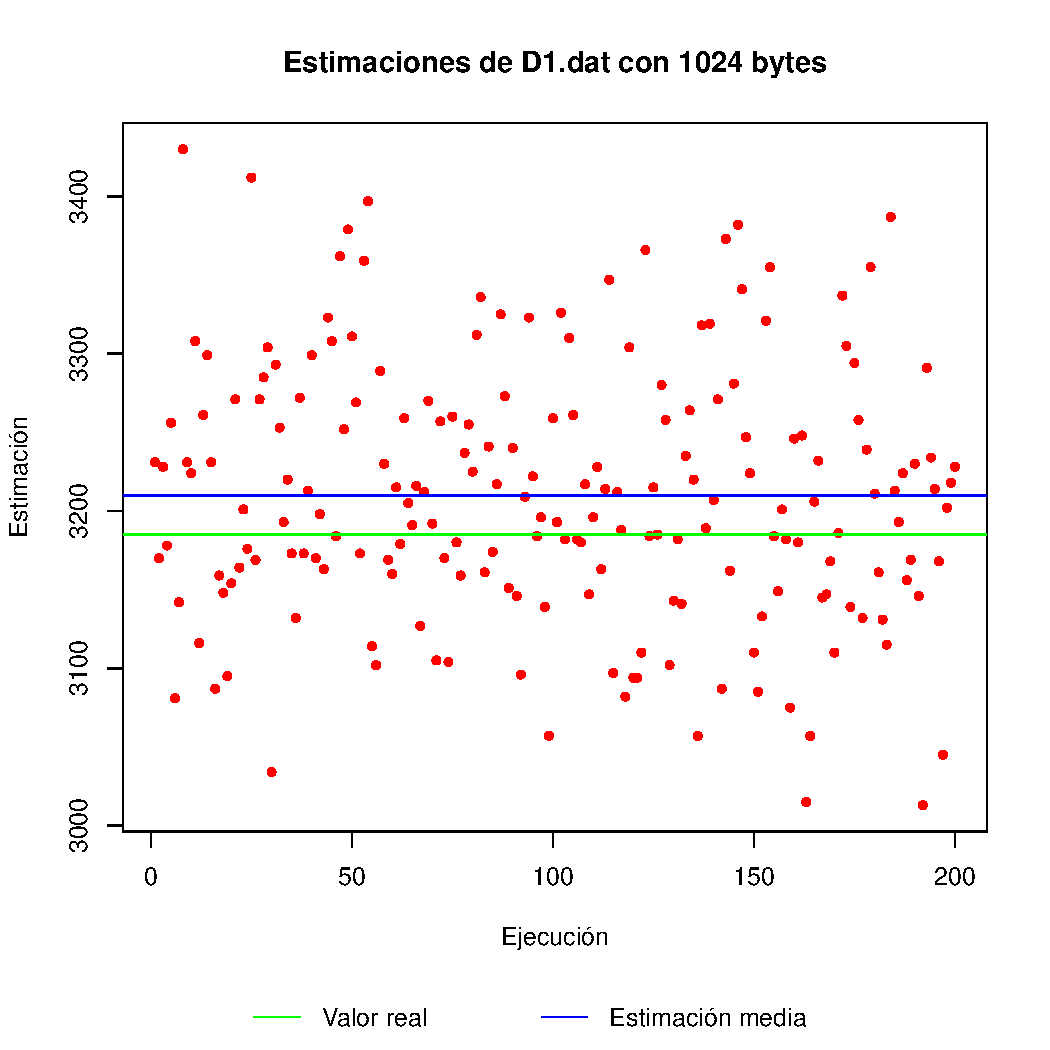
\includegraphics[width=0.64\textwidth]{../figs/D1/plot_estimation_1024.pdf}
        \caption{Estimaciones en D1.dat con 1024 bytes}
    \label{figura:D1_estimation_1024}
\end{figure}

\begin{figure}[h!]
    \centering
        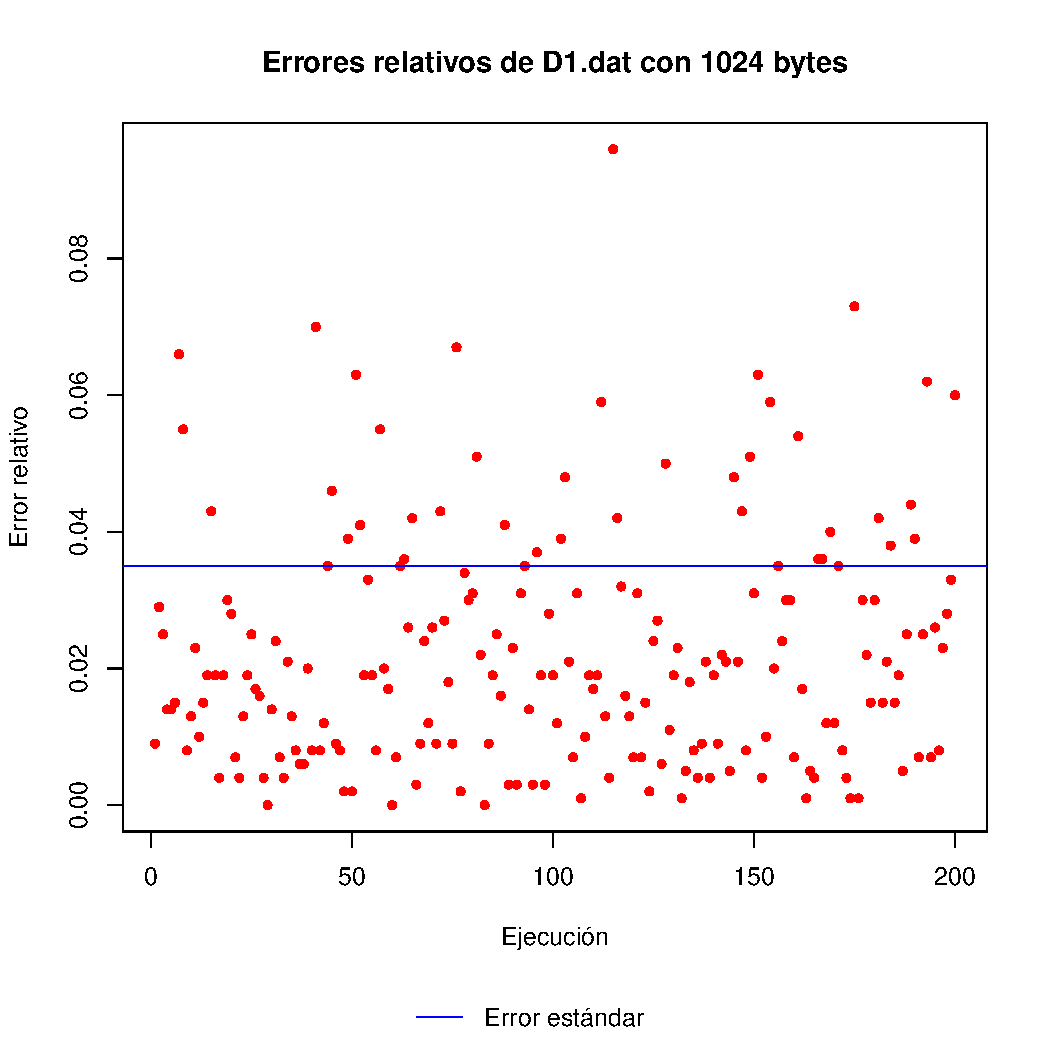
\includegraphics[width=0.64\textwidth]{../figs/D1/plot_errors_1024.pdf}
        \caption{Errores relativos en D1.dat con 1024 bytes}
    \label{figura:D1_errors_1024}
\end{figure}

\begin{figure}[h!]
    \centering
        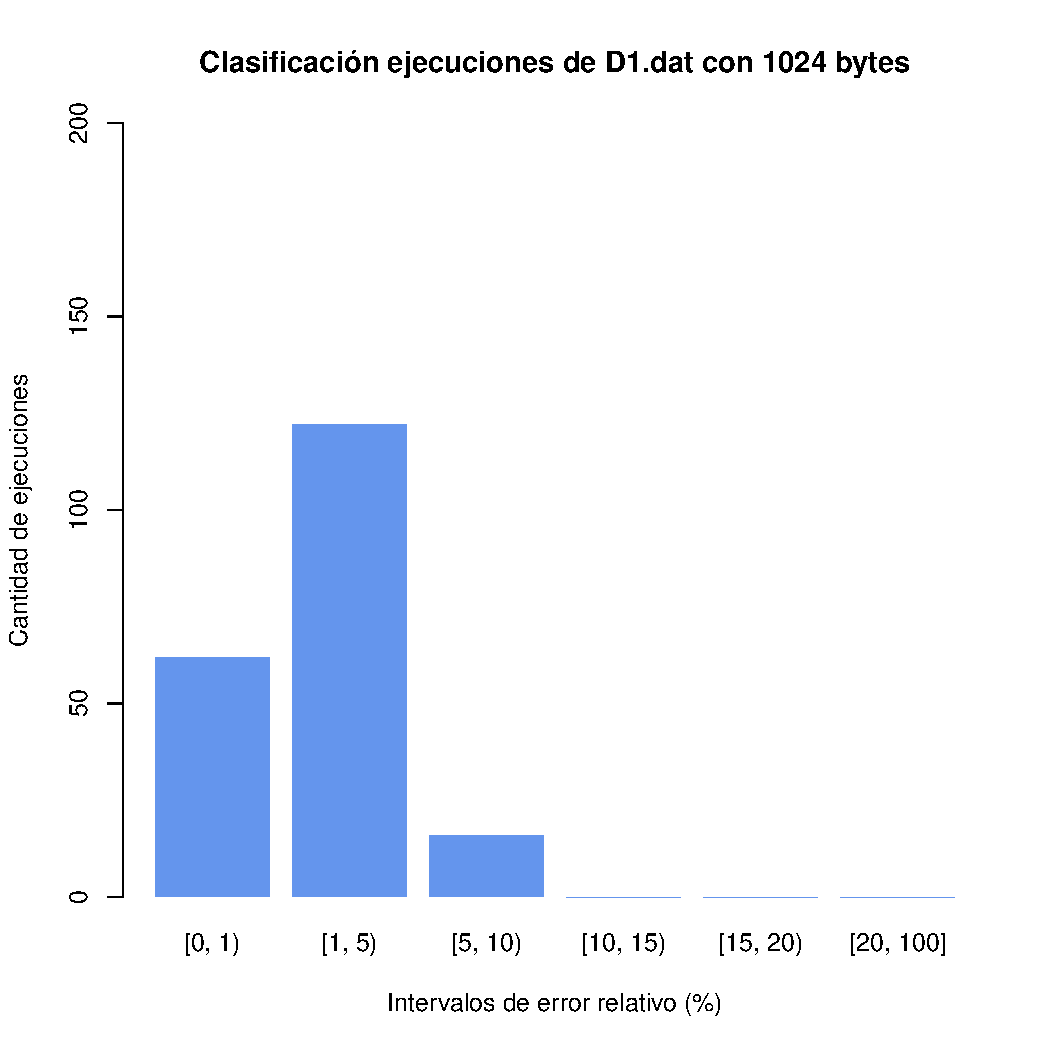
\includegraphics[width=0.64\textwidth]{../figs/D1/plot_count_1024.pdf}
        \caption{Clasificación de ejecuciones en D1.dat con 1024 bytes}
    \label{figura:D1_count_1024}
\end{figure}

\begin{figure}[h!]
    \centering
        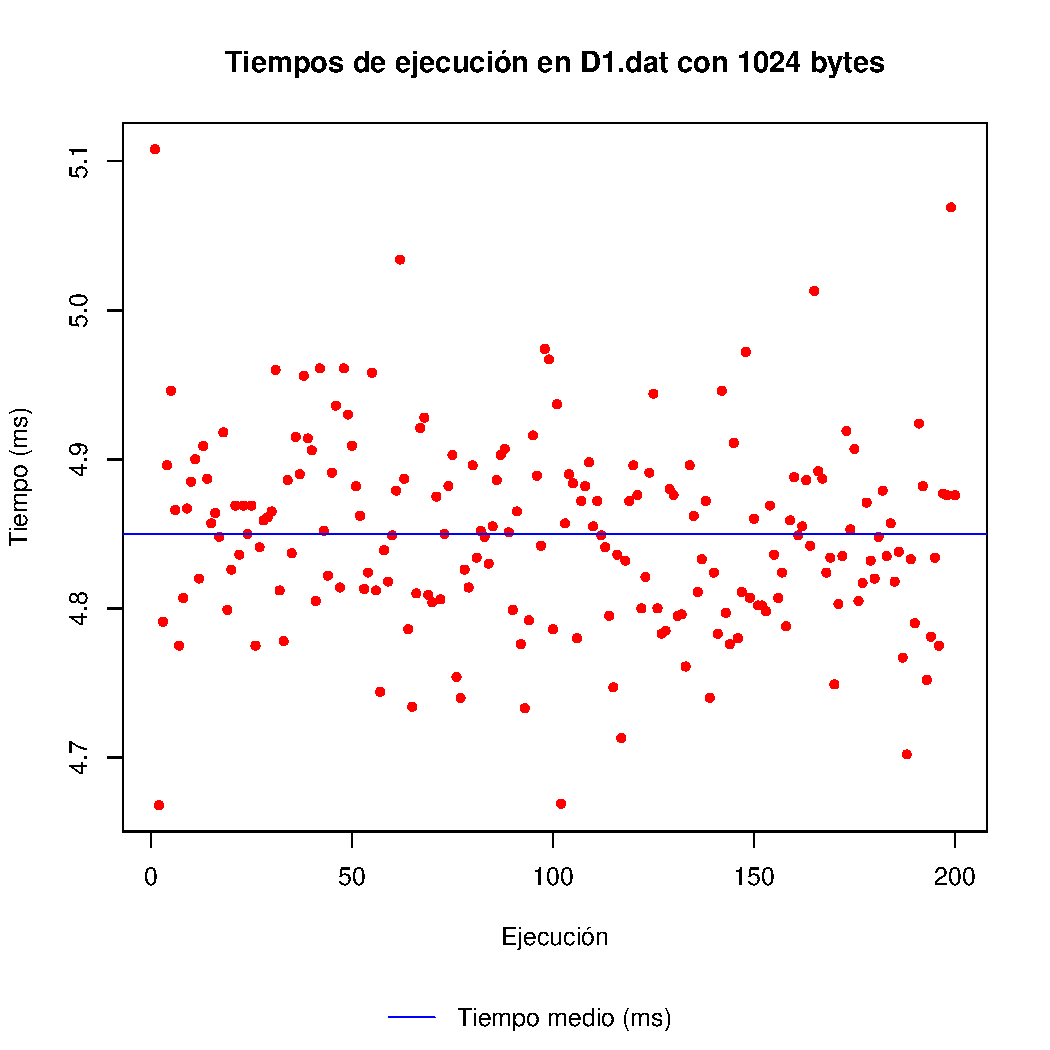
\includegraphics[width=0.64\textwidth]{../figs/D1/plot_time_1024.pdf}
        \caption{Tiempos de ejecución en D1.dat con 1024 bytes}
    \label{figura:D1_time_1024}
\end{figure}

\clearpage
\subsubsection{2048 bytes}
\begin{figure}[h!]
    \centering
        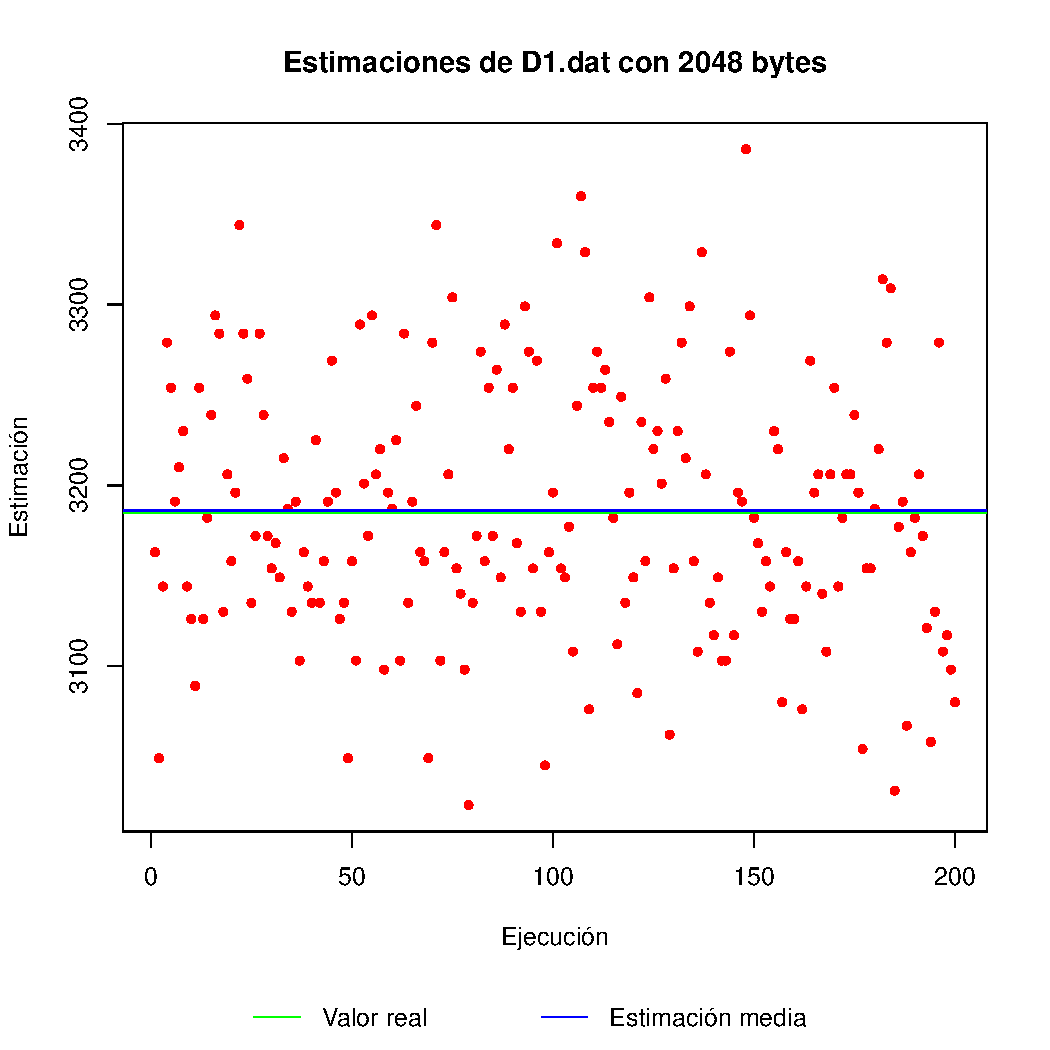
\includegraphics[width=0.64\textwidth]{../figs/D1/plot_estimation_2048.pdf}
        \caption{Estimaciones en D1.dat con 2048 bytes}
    \label{figura:D1_estimation_2048}
\end{figure}

\begin{figure}[h!]
    \centering
        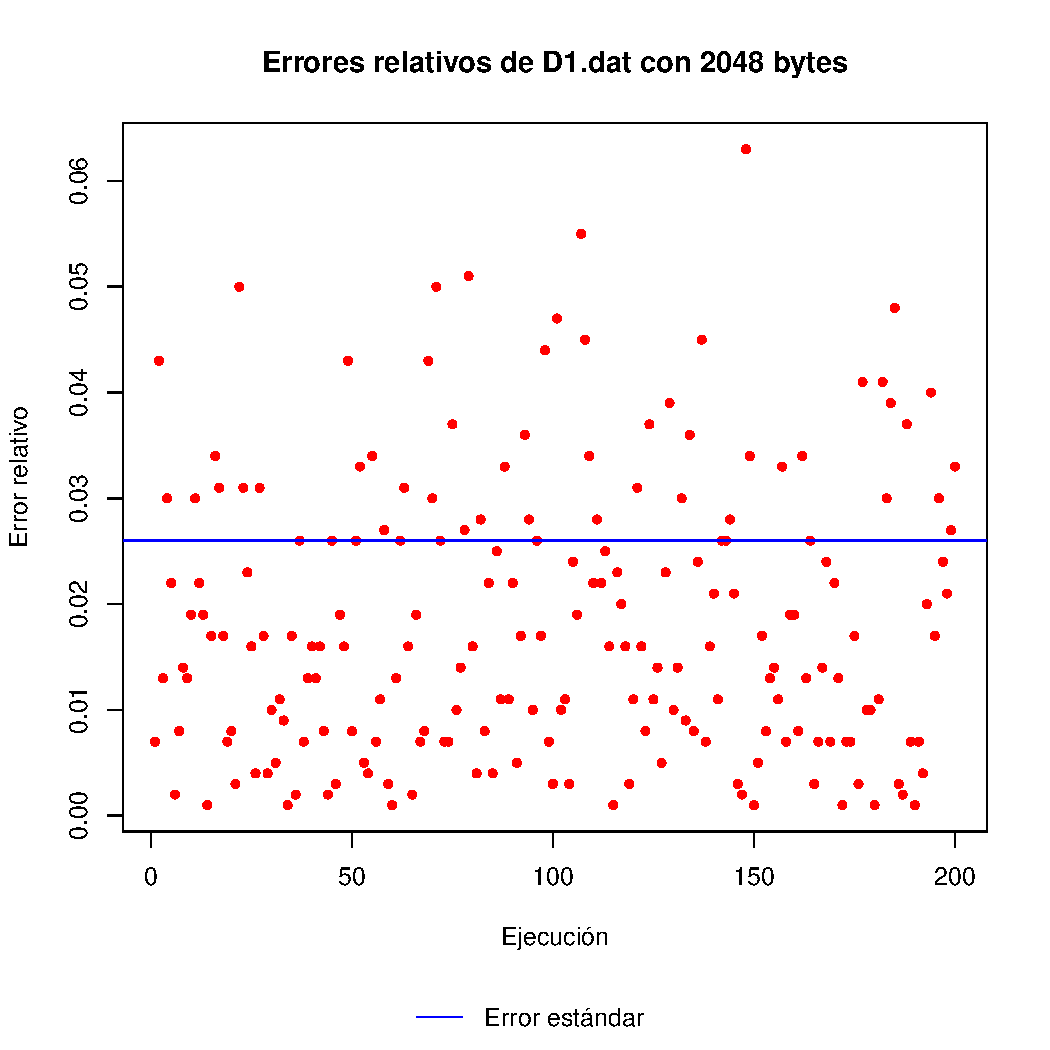
\includegraphics[width=0.64\textwidth]{../figs/D1/plot_errors_2048.pdf}
        \caption{Errores relativos en D1.dat con 2048 bytes}
    \label{figura:D1_errors_2048}
\end{figure}

\begin{figure}[h!]
    \centering
        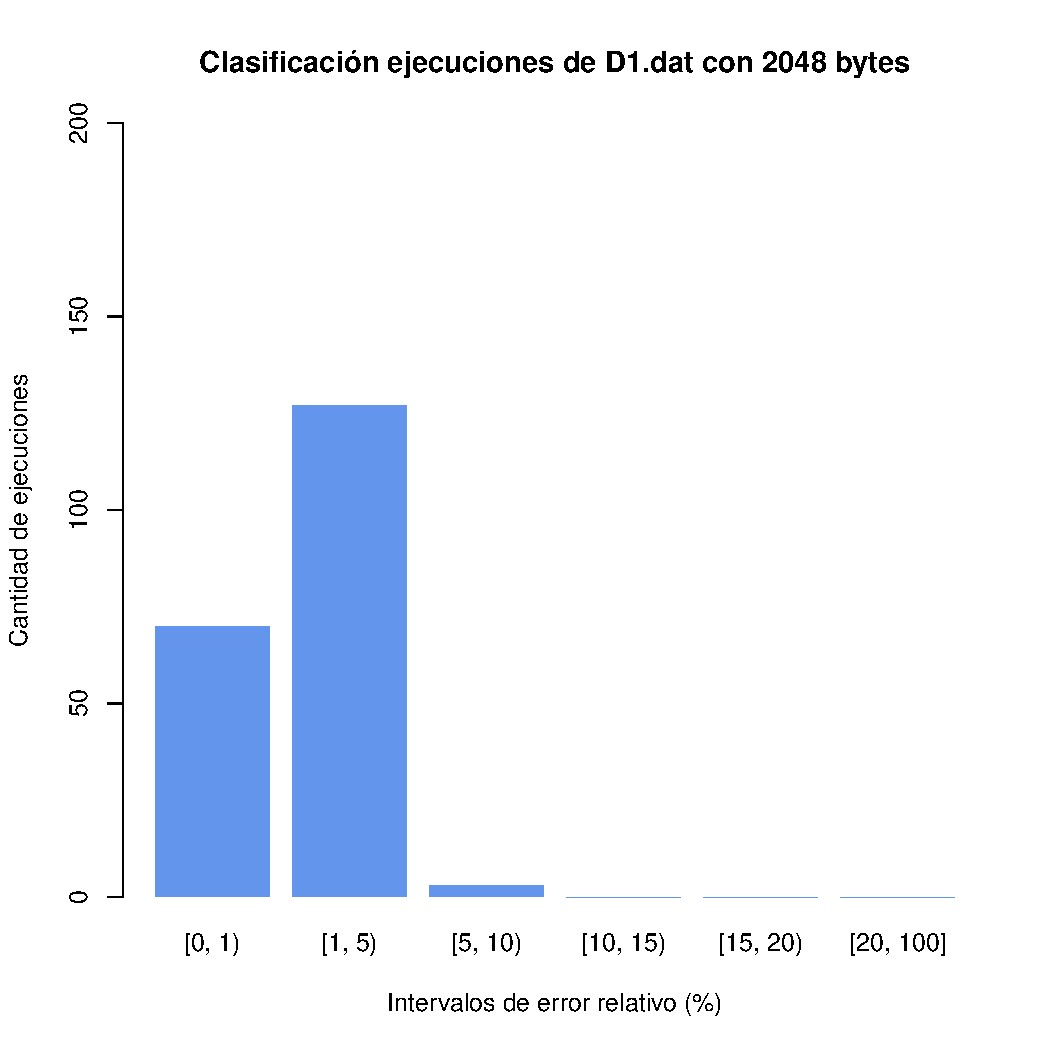
\includegraphics[width=0.64\textwidth]{../figs/D1/plot_count_2048.pdf}
        \caption{Clasificación de ejecuciones en D1.dat con 2048 bytes}
    \label{figura:D1_count_2048}
\end{figure}

\begin{figure}[h!]
    \centering
        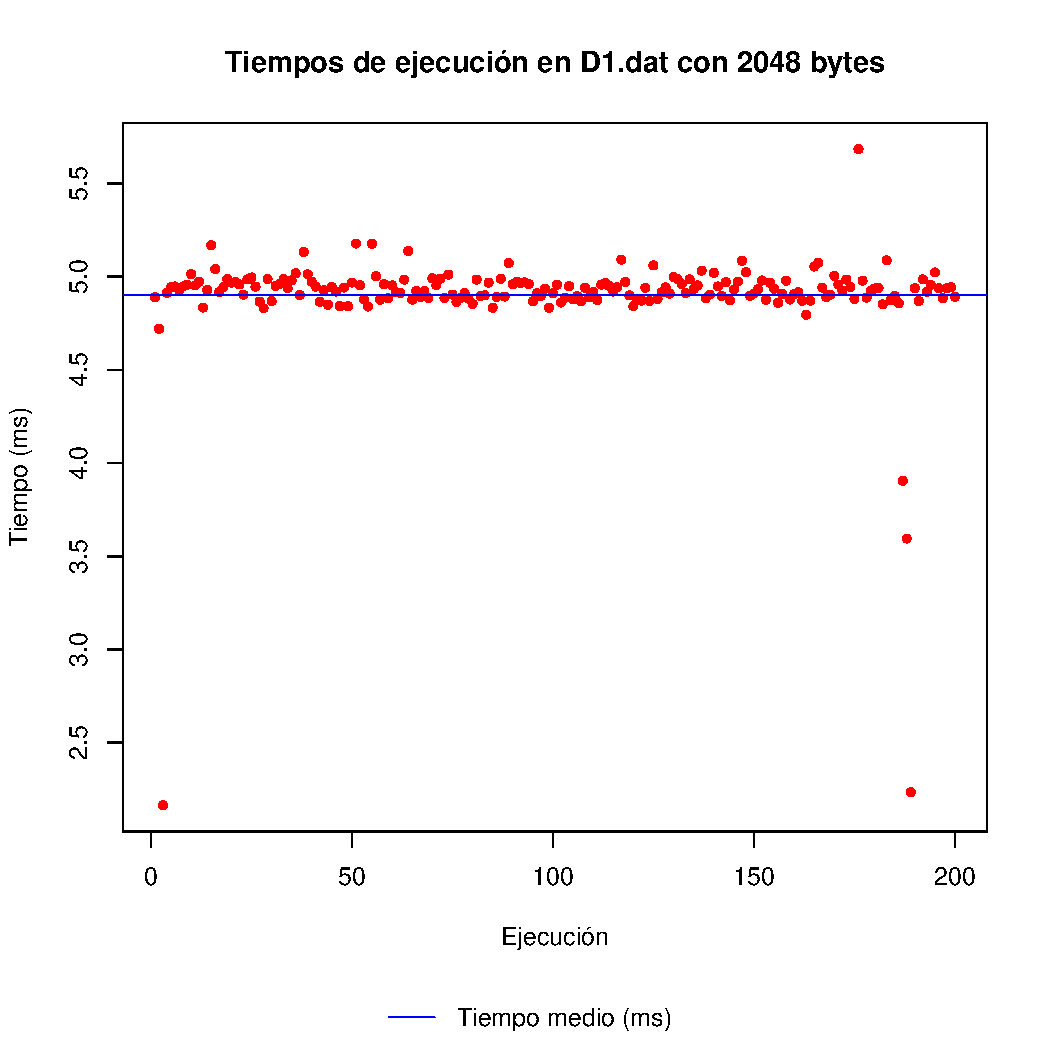
\includegraphics[width=0.64\textwidth]{../figs/D1/plot_time_2048.pdf}
        \caption{Tiempos de ejecución en D1.dat con 2048 bytes}
    \label{figura:D1_time_2048}
\end{figure}

\clearpage
\subsubsection{4096 bytes}
\begin{figure}[h!]
    \centering
        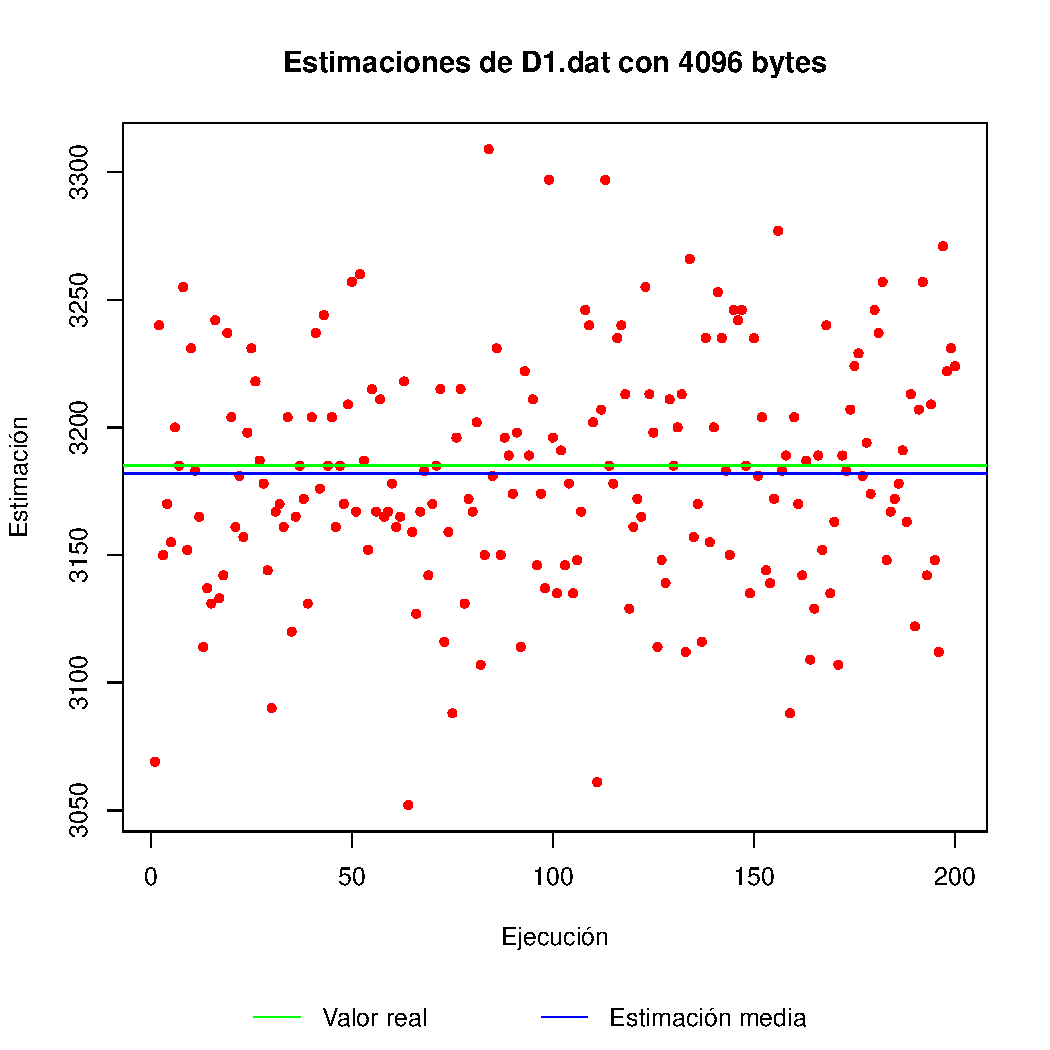
\includegraphics[width=0.64\textwidth]{../figs/D1/plot_estimation_4096.pdf}
        \caption{Estimaciones en D1.dat con 4096 bytes}
    \label{figura:D1_estimation_4096}
\end{figure}

\begin{figure}[h!]
    \centering
        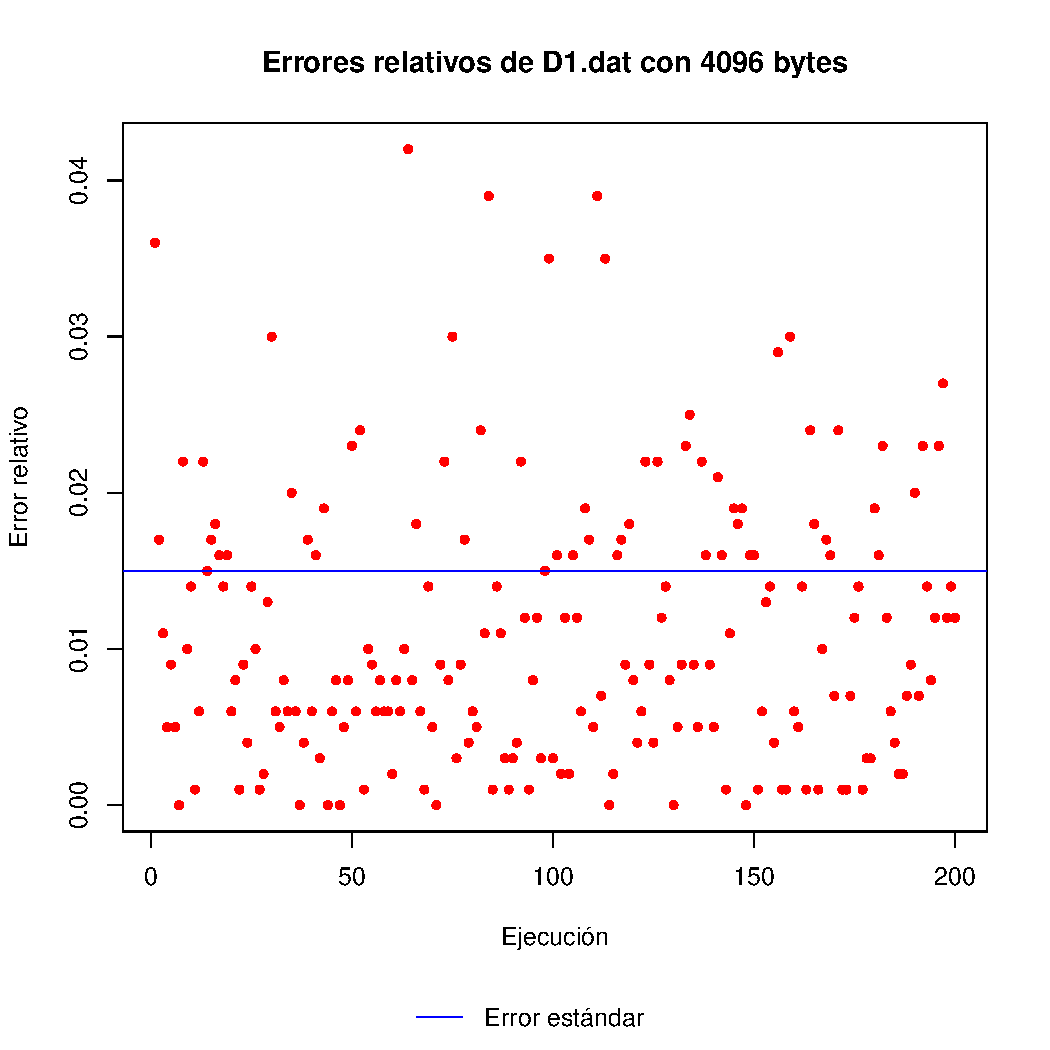
\includegraphics[width=0.64\textwidth]{../figs/D1/plot_errors_4096.pdf}
        \caption{Errores relativos en D1.dat con 4096 bytes}
    \label{figura:D1_errors_4096}
\end{figure}

\begin{figure}[h!]
    \centering
        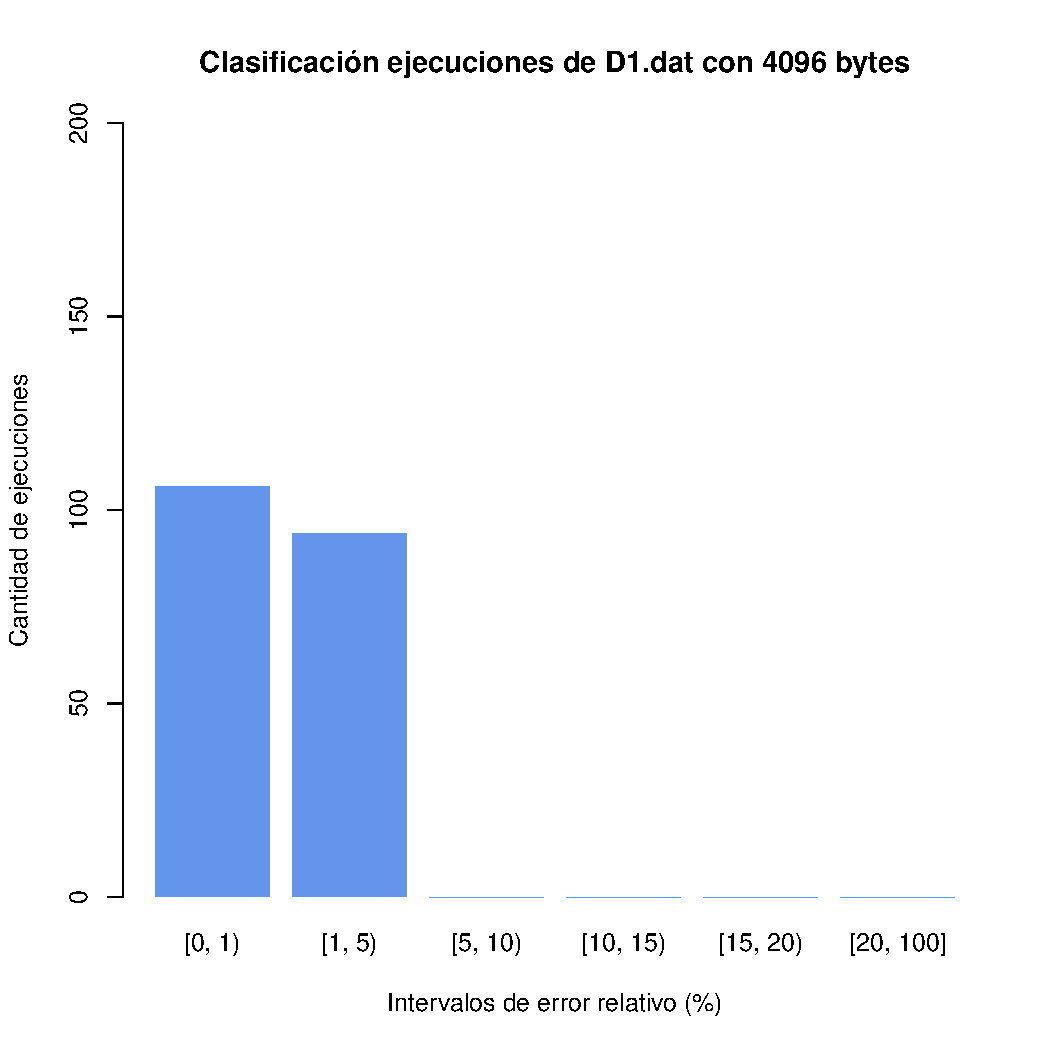
\includegraphics[width=0.64\textwidth]{../figs/D1/plot_count_4096.pdf}
        \caption{Clasificación de ejecuciones en D1.dat con 4096 bytes}
    \label{figura:D1_count_4096}
\end{figure}

\begin{figure}[h!]
    \centering
        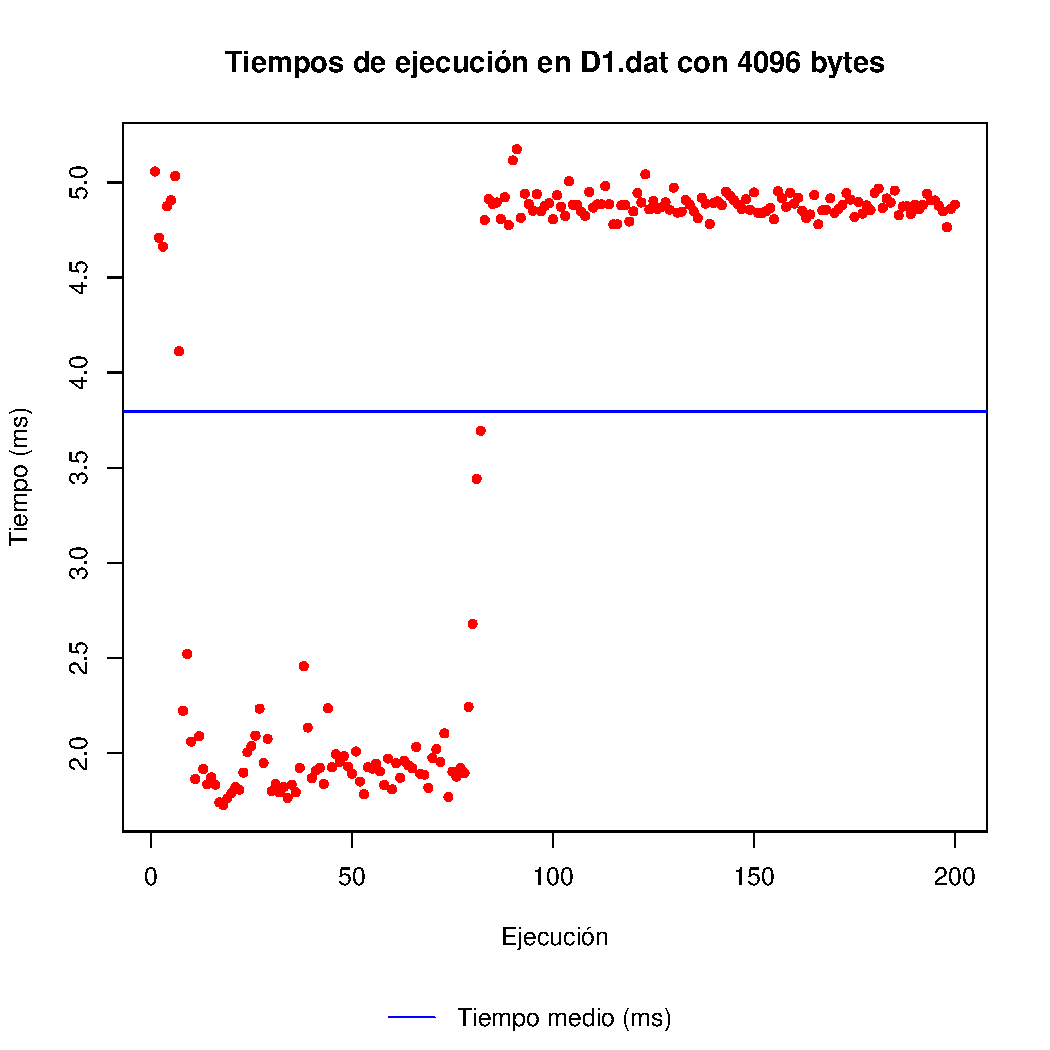
\includegraphics[width=0.64\textwidth]{../figs/D1/plot_time_4096.pdf}
        \caption{Tiempos de ejecución en D1.dat con 4096 bytes}
    \label{figura:D1_time_4096}
\end{figure}

\clearpage
\subsubsection{8192 bytes}
\begin{figure}[h!]
    \centering
        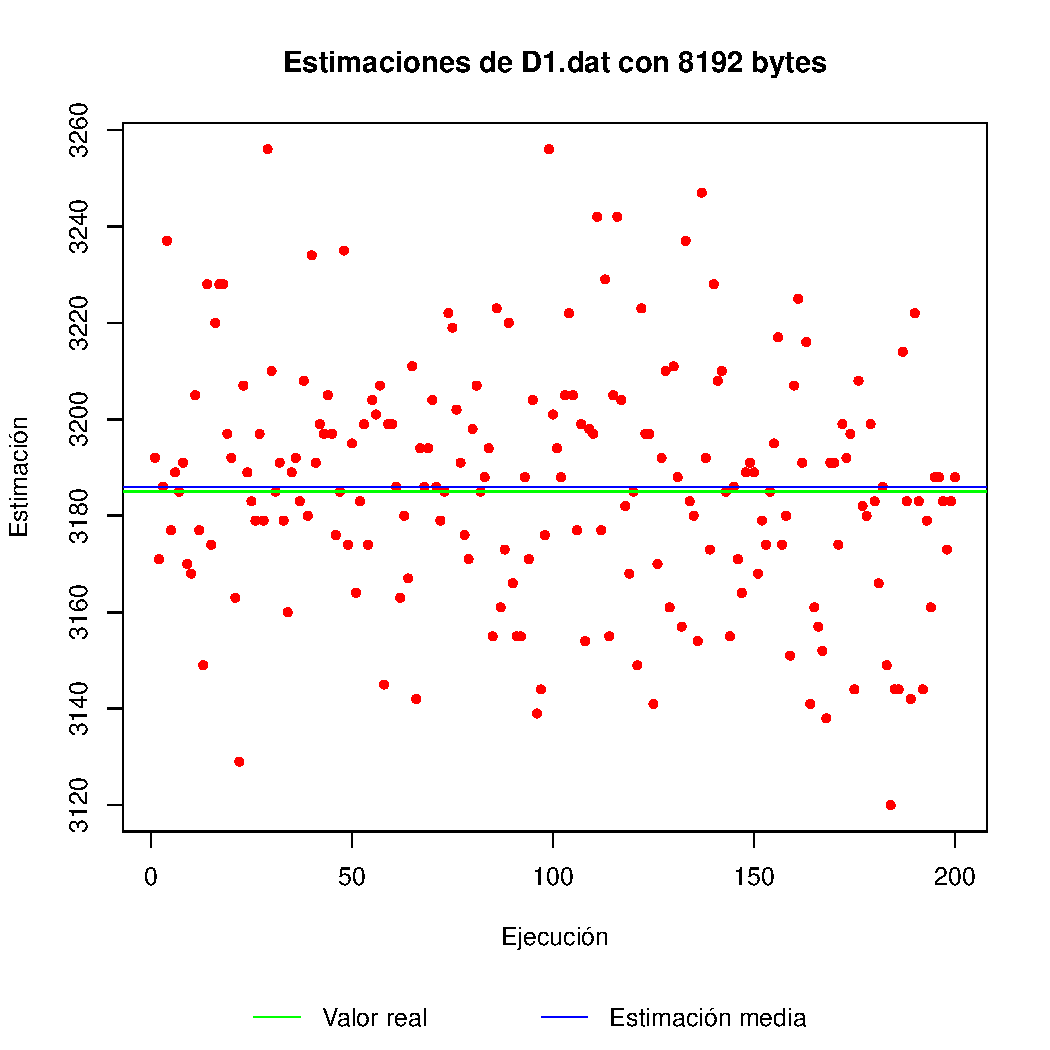
\includegraphics[width=0.64\textwidth]{../figs/D1/plot_estimation_8192.pdf}
        \caption{Estimaciones en D1.dat con 8192 bytes}
    \label{figura:D1_estimation_8192}
\end{figure}

\begin{figure}[h!]
    \centering
        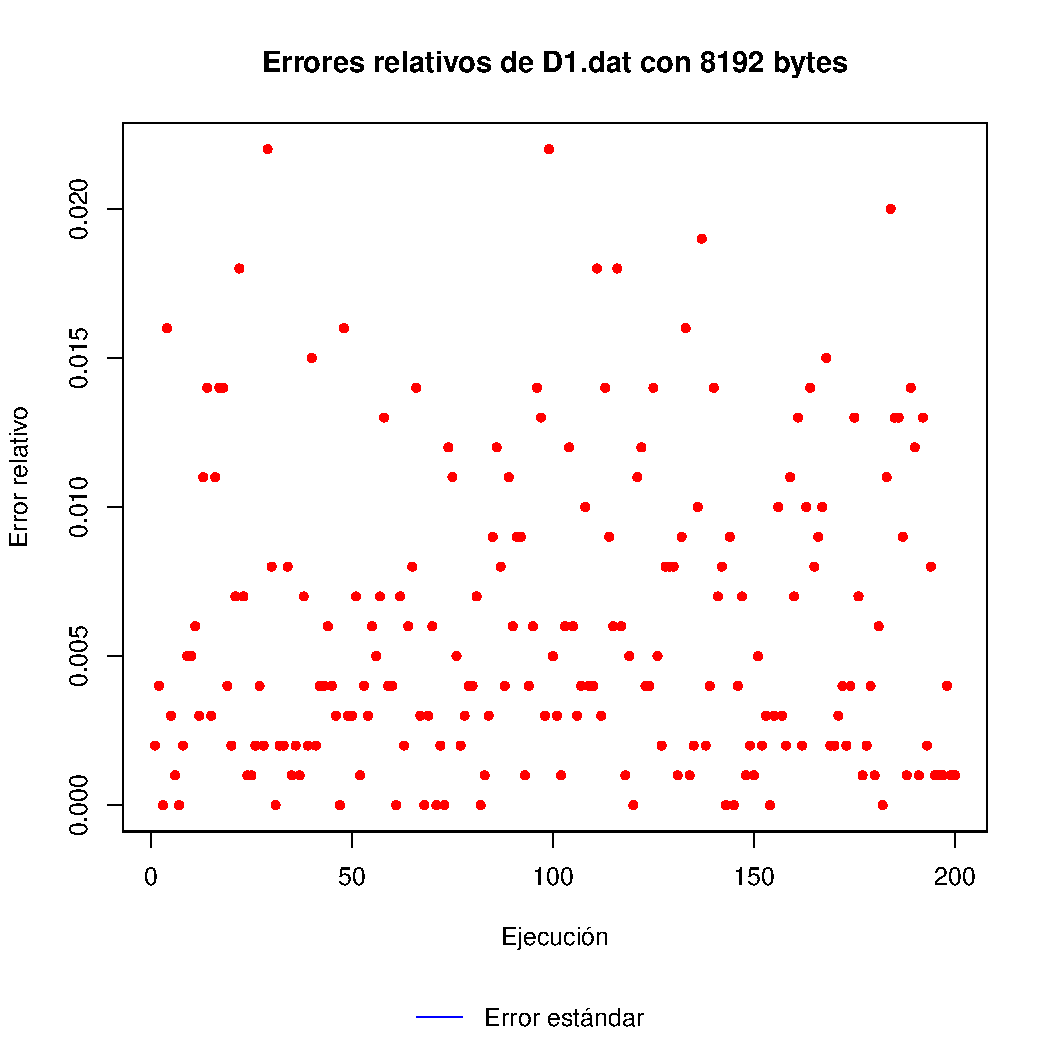
\includegraphics[width=0.64\textwidth]{../figs/D1/plot_errors_8192.pdf}
        \caption{Errores relativos en D1.dat con 8192 bytes}
    \label{figura:D1_errors_8192}
\end{figure}

\begin{figure}[h!]
    \centering
        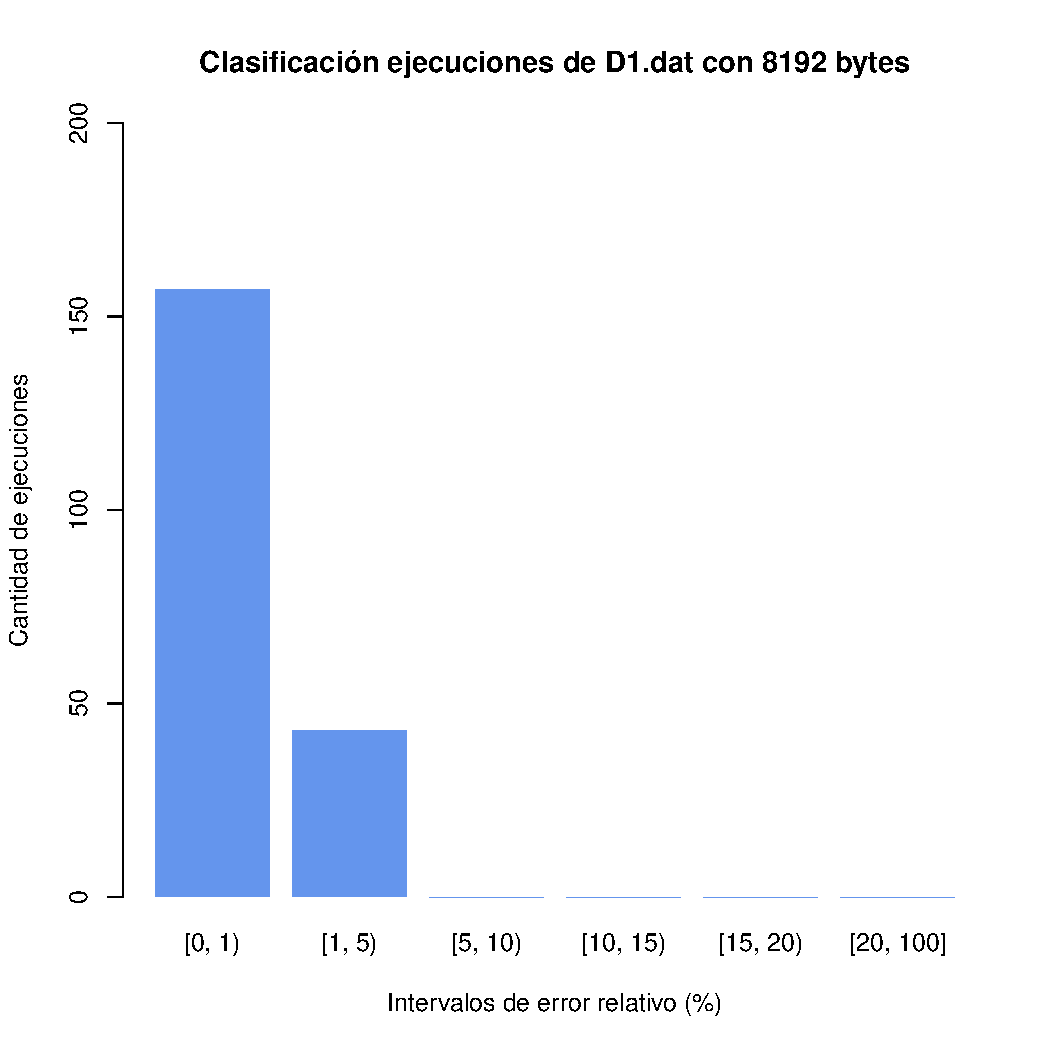
\includegraphics[width=0.64\textwidth]{../figs/D1/plot_count_8192.pdf}
        \caption{Clasificación de ejecuciones en D1.dat con 8192 bytes}
    \label{figura:D1_count_8192}
\end{figure}

\begin{figure}[h!]
    \centering
        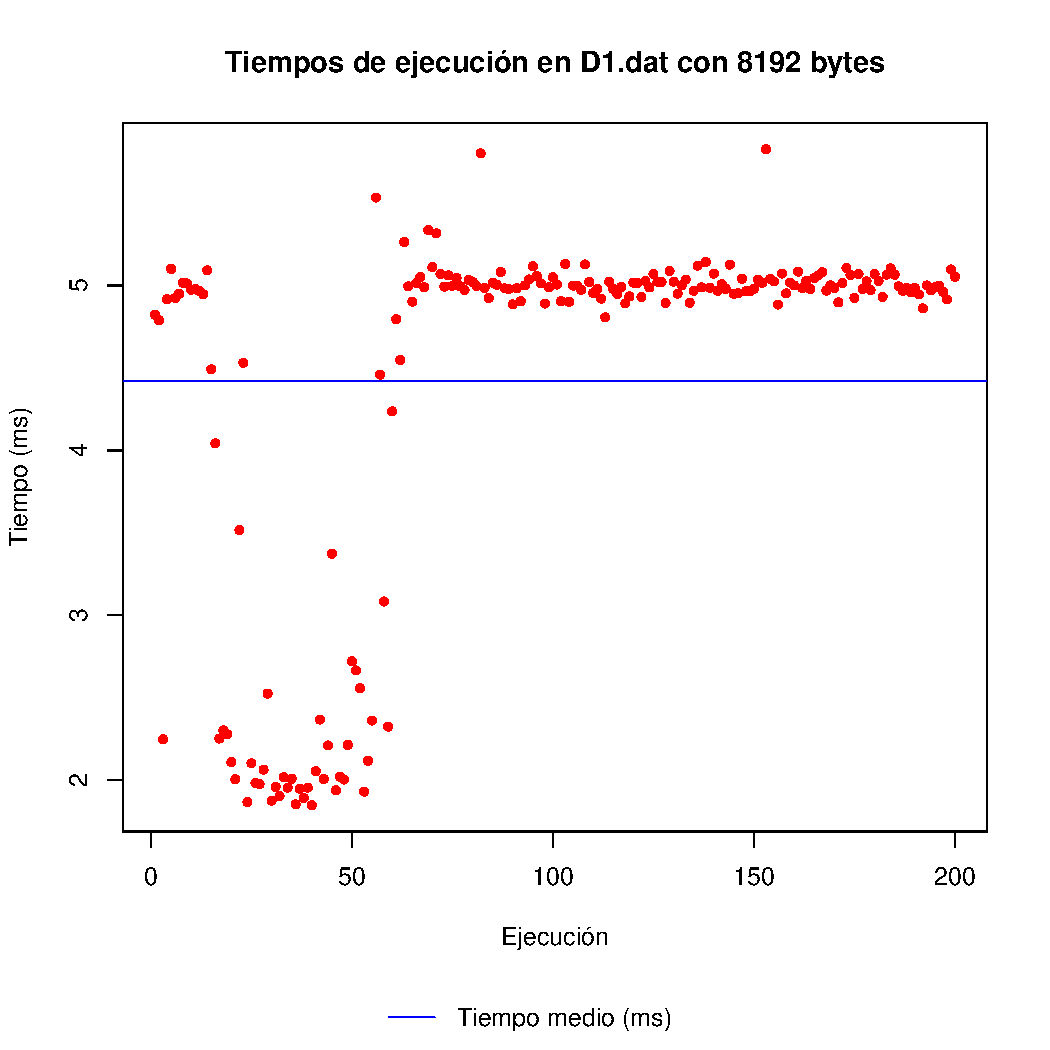
\includegraphics[width=0.64\textwidth]{../figs/D1/plot_time_8192.pdf}
        \caption{Tiempos de ejecución en D1.dat con 8192 bytes}
    \label{figura:D1_time_8192}
\end{figure}

\clearpage
\subsubsection{16384 bytes}
\begin{figure}[h!]
    \centering
        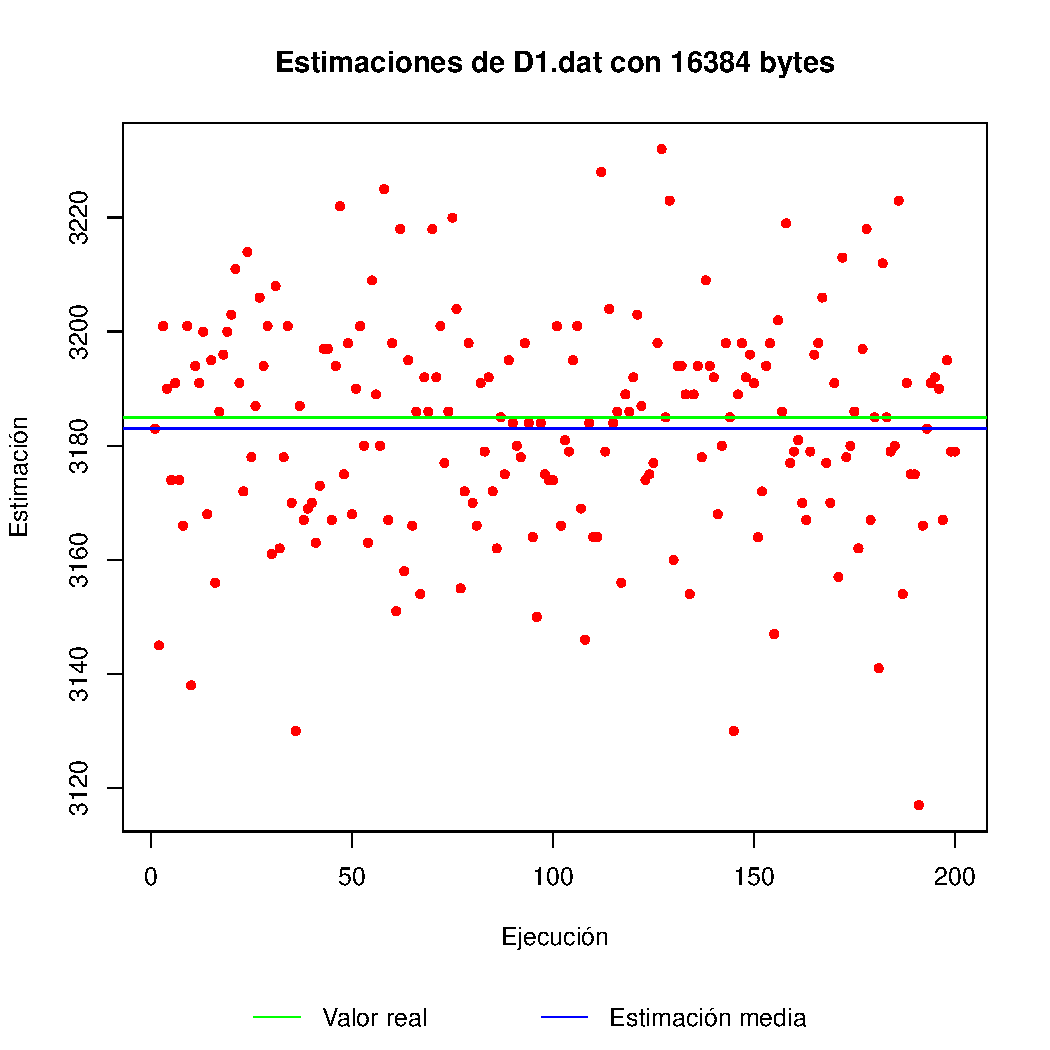
\includegraphics[width=0.64\textwidth]{../figs/D1/plot_estimation_16384.pdf}
        \caption{Estimaciones en D1.dat con 16384 bytes}
    \label{figura:D1_estimation_16384}
\end{figure}

\begin{figure}[h!]
    \centering
        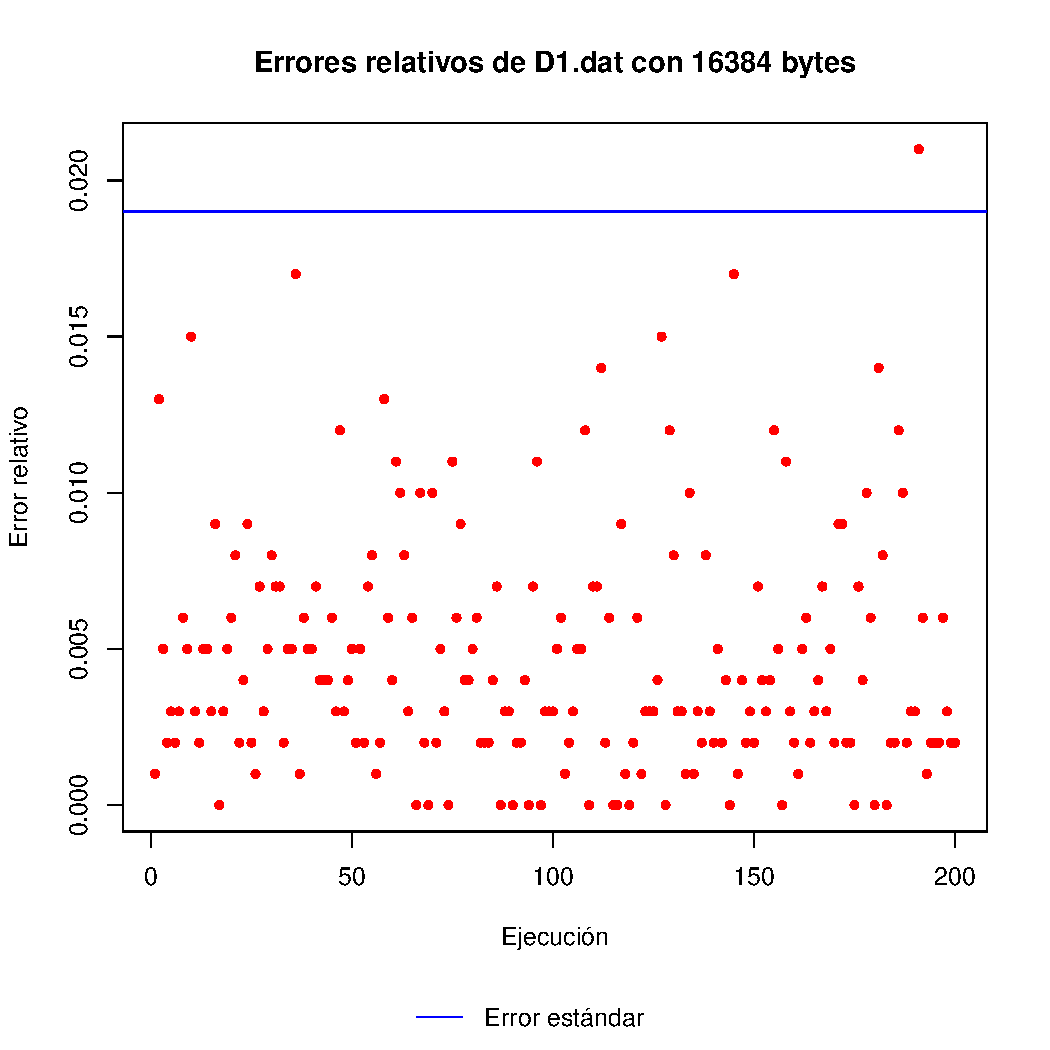
\includegraphics[width=0.64\textwidth]{../figs/D1/plot_errors_16384.pdf}
        \caption{Errores relativos en D1.dat con 16384 bytes}
    \label{figura:D1_errors_16384}
\end{figure}

\begin{figure}[h!]
    \centering
        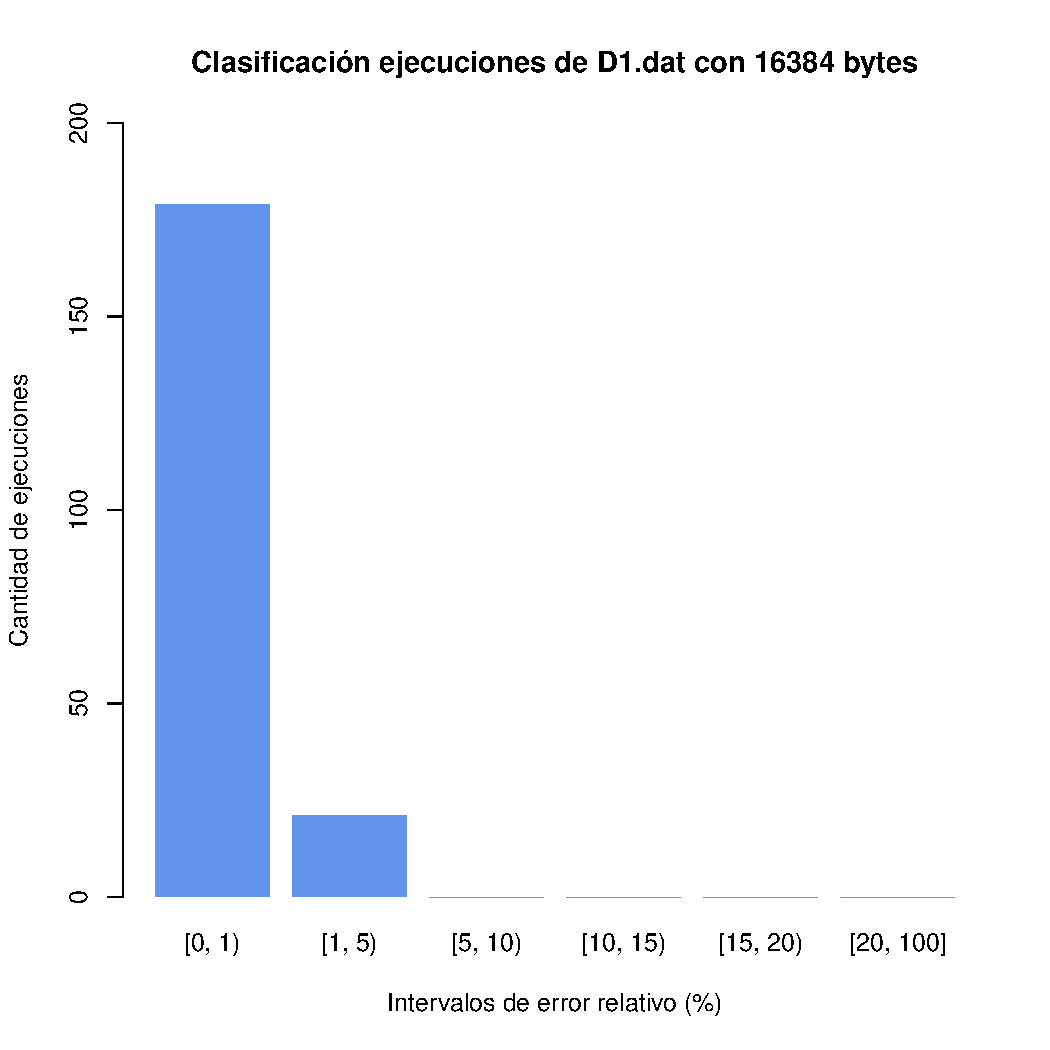
\includegraphics[width=0.64\textwidth]{../figs/D1/plot_count_16384.pdf}
        \caption{Clasificación de ejecuciones en D1.dat con 16384 bytes}
    \label{figura:D1_count_16384}
\end{figure}

\begin{figure}[h!]
    \centering
        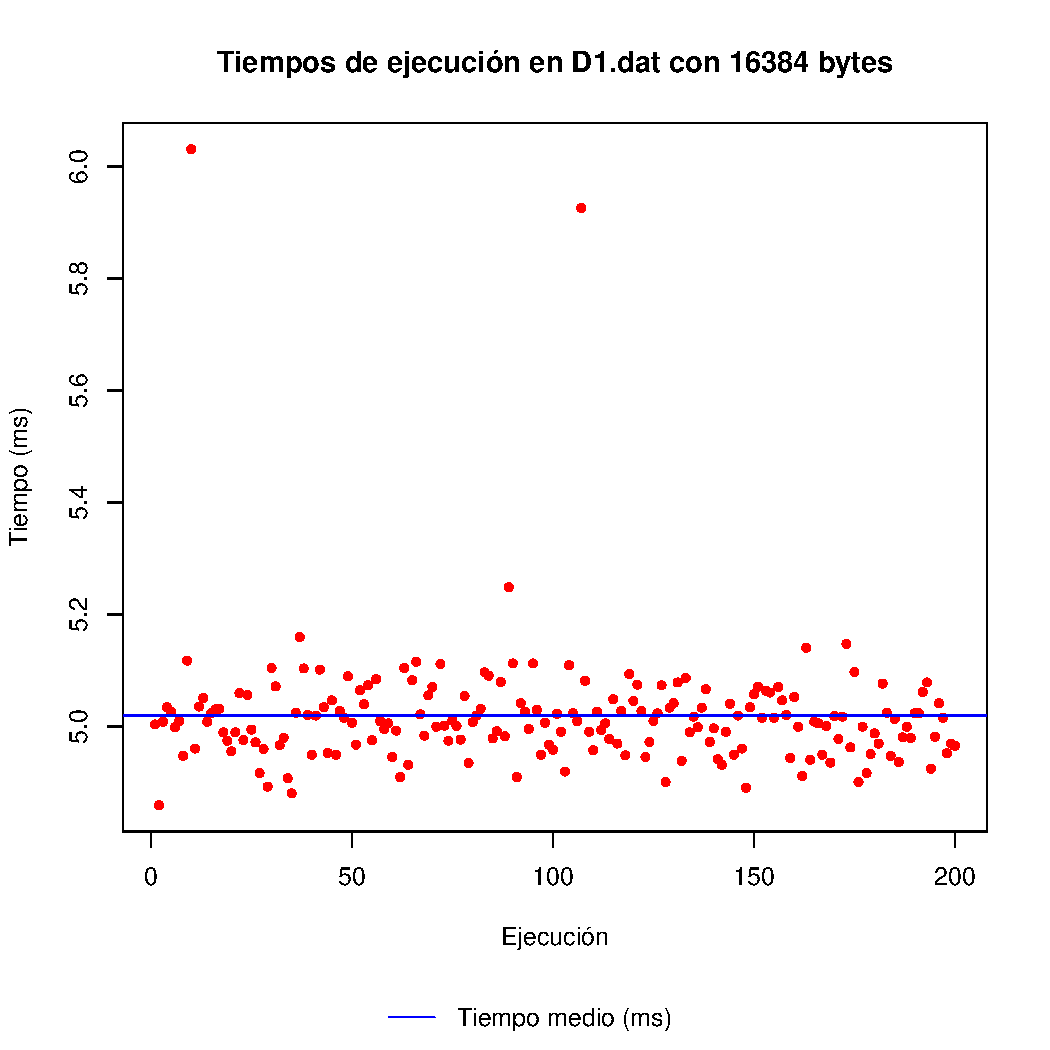
\includegraphics[width=0.64\textwidth]{../figs/D1/plot_time_16384.pdf}
        \caption{Tiempos de ejecución en D1.dat con 16384 bytes}
    \label{figura:D1_time_16384}
\end{figure}

\clearpage

